% TODO mention validation set and test set results
% TODO in discussion comparison to SoA
\chapter{Experiments}
\label{Chapter5}
\settocdepth{subsection}
The majority of our experiments focuses on weighting the watershed locations. That corresponds to the \textbf{Structured voting (SV)} stage of the pipeline SE-SV-UCM, which we propose in \cref{Chapter4} for the task of going from edges to contours.

\textbf{Dataset:} For the evaluation of our segmentation results we work on the Berkeley Segmentation Data Set (BSDS500)~\cite{Arbelaez11}. Since its introduction in 2001, it has by now become a standard dataset for both the task of edge detection as well as that of image segmentation.

\textbf{Benchmark:} We report results on the benchmark~\cite{Galasso13Benchmark} introduced in~\cite{Galasso13} which can evaluate segmentation hierarchies against given ground-truth segmentations. It demonstrates the trade-off between an oversegmentation and a more accurate object-centric segmentation.

\textbf{Watershed weighting strategy:} The Structured voting requires a choice of a watershed weighting strategy. The purpose of the weighting is associating a \textbf{score} with each of the watershed locations pixels. That score must faithfully reflect the strength of the underlying boundary. This way we endeavour % hope % aim, strive %So we want 
to correctly evaluate how good is the boundary evidence presented by the most likely segmentation - the one determined by the structured forest. 

The first aspect of our voting strategy is making the structured forest patch and the watershed locations patch comparable. The watershed patch is an oversegmentation, and in this sense, contains much more information, not exclusively about the location of the boundary that we would like to evaluate. So we strive to simplify the watershed patch, keeping only important information about it - the shape of the boundary under consideration, or the constitution of the segmentation in the patch. Such a simplification in the context of our algorithm we call {\bf watershed patch transformation}. %``watershed patch transformation''. 

The second particular to a watershed weighting strategy is the choice of a scoring function. We view the task as a segmentation benchmark problem, where one of the patches is the ground truth segmentation, and the other - the segmentation under test. We analyse and apply a selection of boundary- and region- based metrics.

In the rest of the chapter we briefly describe the dataset and evaluation metrics used, in order to help understand the experiments. Afterwards, we give a detailed account of our most important experiments and the conclusions we draw based on them.

\section{Evaluation setup} % framework, organisation
\subsection{Dataset}
\label{sec:ch5-BSDS500-dataset}
\subsubsection{BSDS500}
The Berkeley Segmentation Data Set (BSDS), introduced in \cite{Martin01}, is a large dataset that covers a variety of complex scenarios in natural images. The photographs have been manually segmented by multiple participants. It, therefore, provides the ground truth label for each pixel as being on- or off-boundary. Initially the dataset featured 300 images (BSDS300). It was later extended - in the new dataset BSDS500 \cite{Arbelaez11} the original 300 images are used for training (200) and validation (100), and 200 new human-annotated images are added for testing. Again, each image has 5 to 10 hand-drawn annotations by different subjects. See \fref{fig:BSDS-annotations} for an example image and two of its ground-truth segmentations. %annotations by different people.

BSDS is a widely used benchmark for both boundary detection and general image segmentation.

\begin{figure}[ht!]
\begin{center}
  \begin{tabular}{ c c c }
  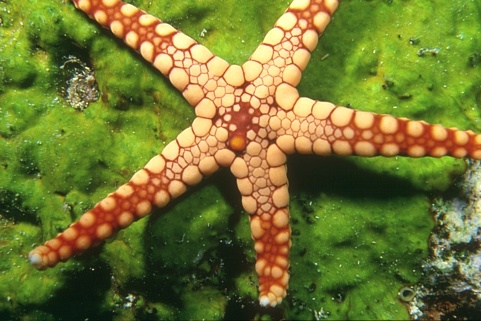
\includegraphics[width=0.3\textwidth]{images/examples/starfish/starfish.png} &
  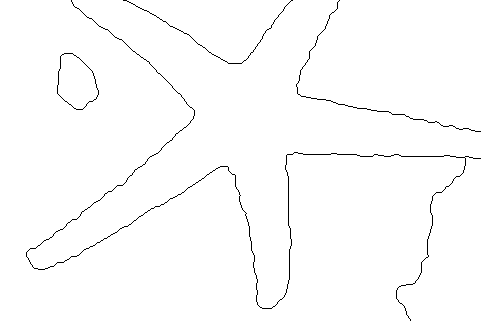
\includegraphics[width=0.3\textwidth,frame]{images/examples/starfish/starfish_bdry_coarse.png} &
  
\includegraphics[width=0.3\textwidth]{images/examples/starfish/starfish_segm_coarse.png} \\
  &
  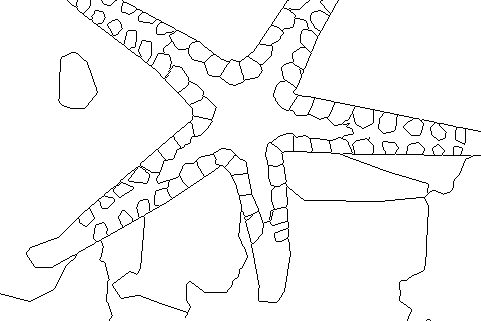
\includegraphics[width=0.3\textwidth,frame]{images/examples/starfish/starfish_bdry_detail.png} &
  
\includegraphics[width=0.3\textwidth]{images/examples/starfish/starfish_segm_detail.png} \\
  Input image & Boundaries & Segmentation \\
  \end{tabular}
\end{center}
\caption[BSDS500 dataset - 2 annotations]{Image from the validation subset of~\cite{BSDS500resources} and two of its annotations - subject~1 on the first row, subject~2 on the second row. {\bf Human-marked boundaries} are the central column, and their corresponding {\bf segmentation} reconstructions are given next to them.}
\label{fig:BSDS-annotations}
\end{figure}

\subsubsection{Difficulty of the dataset}
It is worth, perhaps, pointing attention to the challenge that this dataset presents.

According to Gestalt psychologists \cite{Wertheimer1923untersuchungen,Kohler1929task,Koffka1935principles,Wertheimer1938laws}, human visual grouping is influenced by several common factor (\eg similarity, continuity, parallelism, closure, familiarity). Nevertheless, as we discussed in \sref{sec:ch1-problem-challenges}, different people have different understanding as to the relevant degree of detail for an image. 

In an attempt to capture this variability in what people perceive as a ``natural'' segmentation, Martin \etal \cite{Martin01} only gave vague instructions to the BSDS annotators: \begin{quote}Divide each image into pieces, where each piece represents a distinguished thing in the image. It is important that all of the pieces have approximately equal importance. The number of things in each image is up to you. Something between 2 and 20 should be reasonable for any of our images.\end{quote}

Consequently, annotations sometimes greatly differ in the level of granularity, see \fref{fig:sub:BSDS-perceptual-different} (but still {\it mostly} agree on boundary localisation). Also, they are typically more fine-grained than the basic %simplest 
figure vs. ground assignment (see the blue nodes of the tree on \fref{fig:sub:BSDS-perceptual-perceptual-organisation-tree}) that some tasks require \cite{Ren2006figure,Sundberg2011occlusion}.

\begin{figure}[ht!]
\centering
 \subfigure[BSDS images each alongside 2 annotations - a coarse and a detailed one]{%
  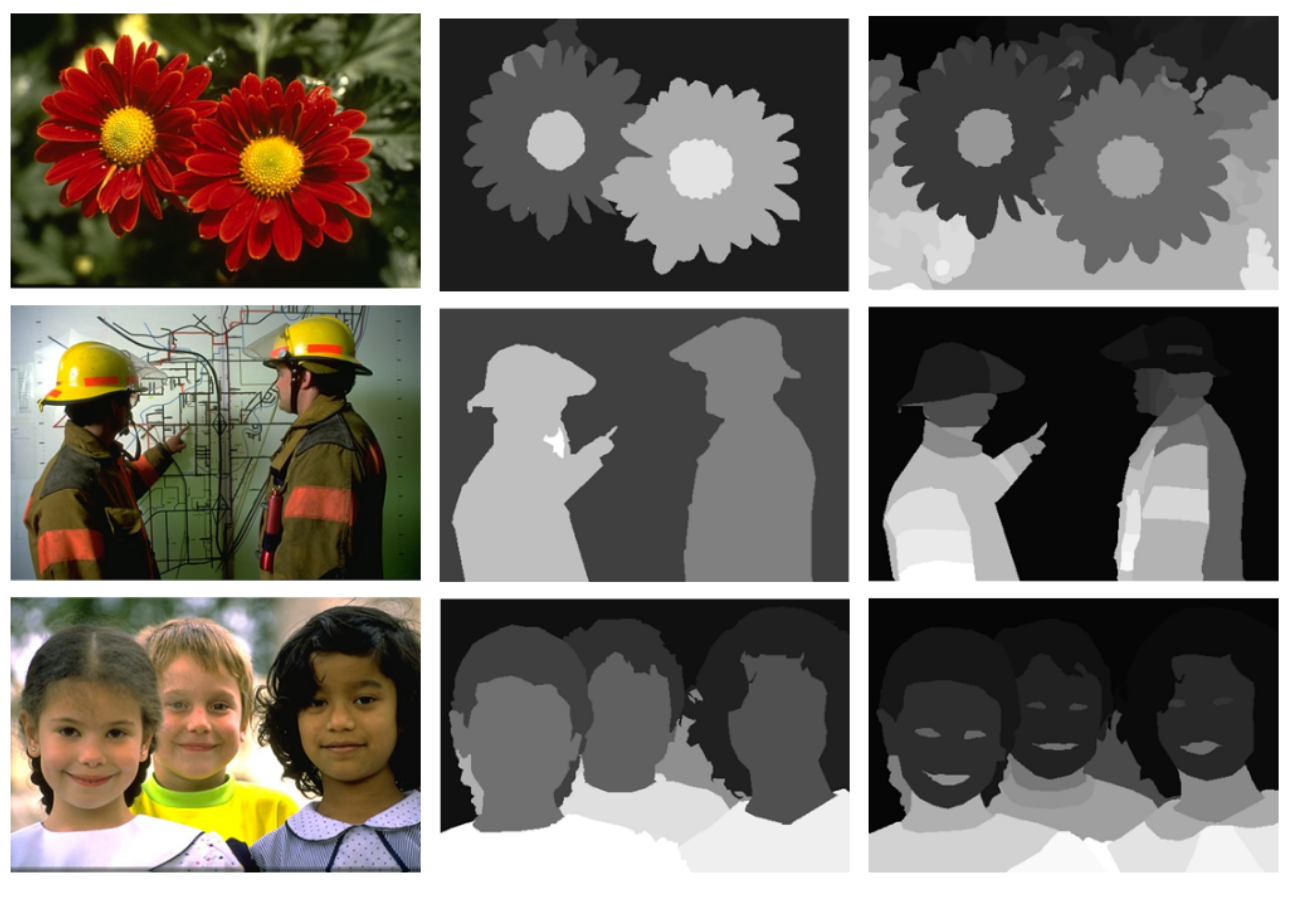
\includegraphics[width=0.4\textwidth]{images/BSDS/Li2013SemanticBenchmark-different-annotations-examples.png}
  \label{fig:sub:BSDS-perceptual-different}
 }
 \subfigure[Perceptual organisation of an image]{%
  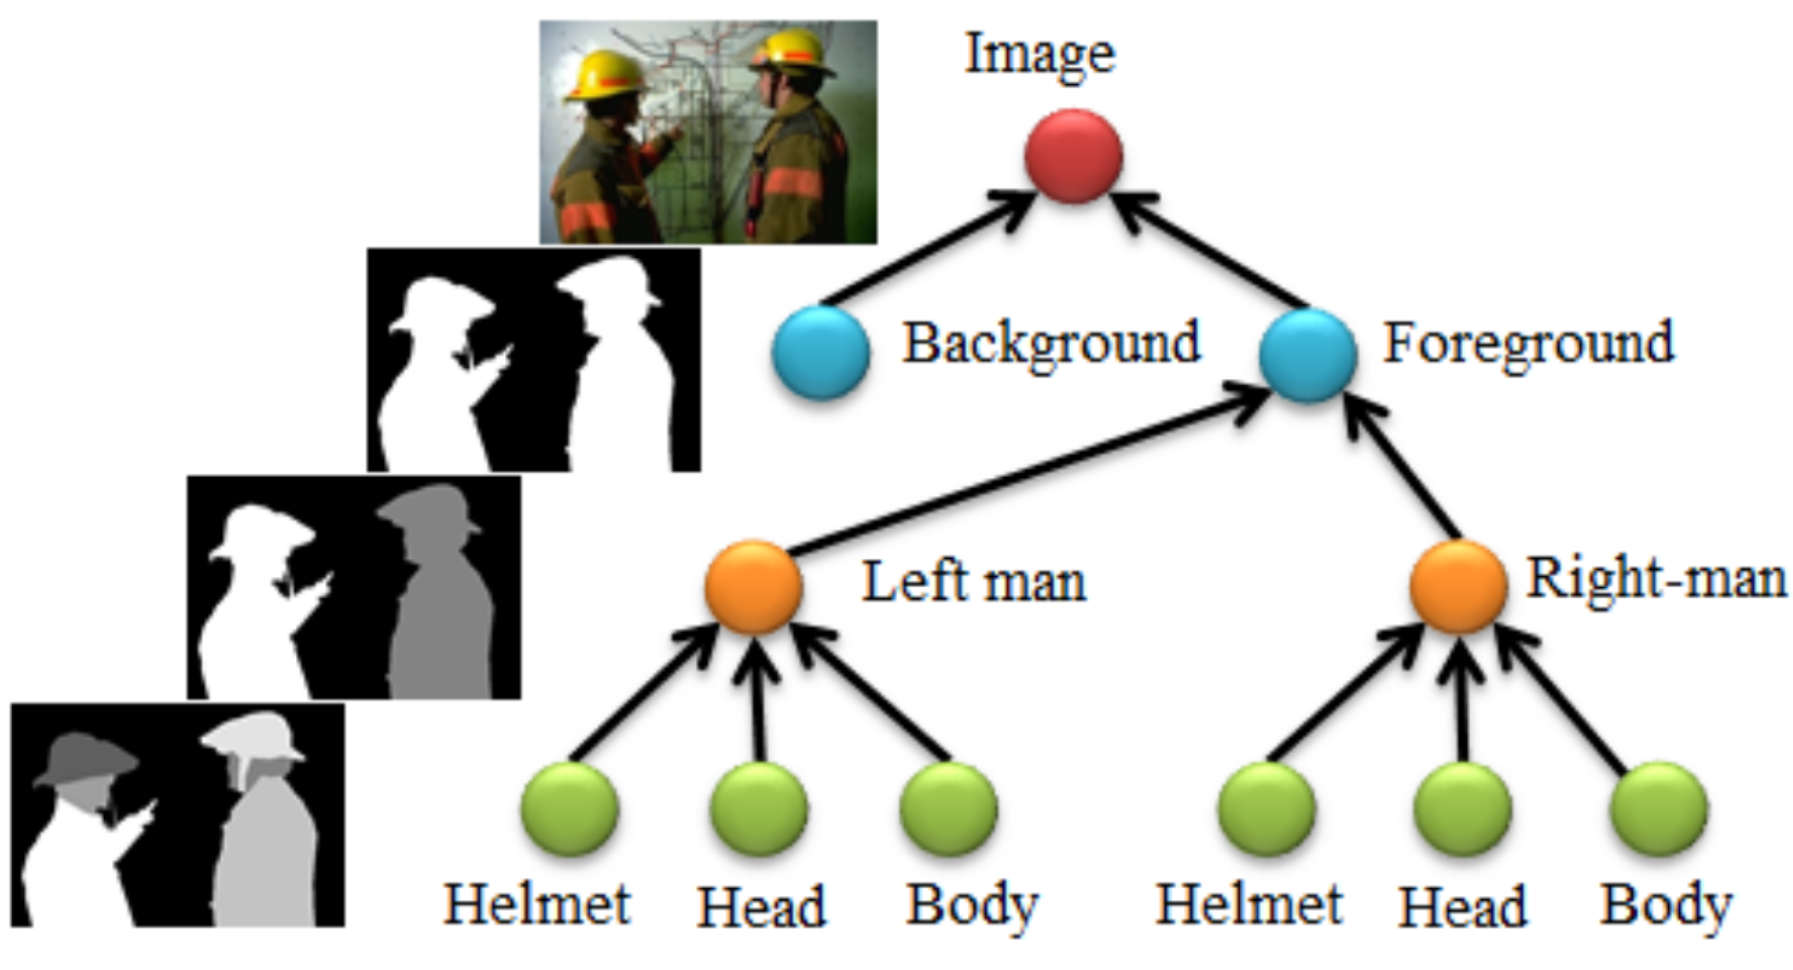
\includegraphics[width=0.57\textwidth]{images/BSDS/Li2013SemanticBenchmark-perceptual-organisation-tree.png}
  \label{fig:sub:BSDS-perceptual-perceptual-organisation-tree}
 }
\caption[Difficulty of BSDS - differences in the perceptual organisation of a scene]{Difficulty of BSDS - differences in the perceptual organisation of a scene. Images courtesy of \cite{Li2013SemanticBenchmark}.}
\label{fig:BSDS-perceptual}
\end{figure}

\subsection{Evaluation metrics}
\settocdepth{section}
The benchmark that we use provides, among others, two precision-recall metrics - a boundary and a region oriented one.

% from \cite{Arbelaez11}
%- One option is to regard the segment boundaries as contours and evaluate them as such. However, a methodology that directly measures the quality of the segments is also desirable. Some types of errors, e.g., a missing pixel in the boundary between two regions, may not be reflected in the boundary benchmark,but can have substantial consequences for segmentation quality, e.g., incorrectly merging large regions. One might argue that the boundary benchmark favours contour detectors over segmentation methods since the  former  are  not  burdened  with  the  constraint  of producing  closed  curves.  We  therefore  also  consider various region-based metrics.

\subsubsection{BPR}
\label{sec:ch5-BPR-evaluation-metric}
The Boundary Precision-Recall (BPR)~\cite{Arbelaez11} is a boundary-based metric and emphasises the correct placement of image edges. Section~\ref*{sec:ch4-boundary-and-region-metrics-maths}~\ref{par:ch4-BPR-maths} % avoid having both links by using ref*
gives mathematical account on the metric and its properties. In case of segmentation, BPR is a good indicator of the {\bf localisation of the region boundaries}.

\textbf{Impact of %small 
local change in the boundary on the score:} A difference in the score of a single region boundary pixel should not greatly affect the edge detector output. Therefore, it correctly has only a small impact on the BPR metric. For the task of image segmentation however, a change in the strength of a single pixel could result in merging neighbouring regions. A ``weaker'' pixel among a strong intervening boundary could be thought of as a leakage, which will cause the UCM algorithm (featured in \sref{sec:ch3-UCM}) % TODO give the algorithm in an appendix
to merge the two regions. In the hierarchical image segmentation framework, that means multiple levels of the segmentations hierarchy would change. Therefore a rigorous image segmentation benchmark metric should not be oblivious to such changes.

\subsubsection{VPR}
To address the above issue, the other metric that we report is the Volume Precision-Recall (VPR) introduced by Galasso \etal~\cite{Galasso13} to evaluate the accuracy of video segmentation algorithms. For images (or video still frames) the metric is a region-based metric, operating % applied
into a precision-recall framework. It is measuring the size of the regions and the overlap between the ground truth segmentation regions and the segmentation regions produced by the algorithm under test. 
See Section~\ref*{sec:ch4-boundary-and-region-metrics-maths}~\ref{par:ch4-VPR-maths} for the formulae and discussion on the need for normalisation when evaluating segmentations.

\subsubsection{Reported numbers}
\paragraph{For the precision-recall metrics BPR and VPR}\mbox{}\\\mbox{}\\
Both BPR and VPR are able to evaluate {\bf individual segmentations} (which on the plots are depicted as a single dot - the model error), as well as {\bf segmentation hierarchies}, represented using the UCM data structure (which on the plots constitute a curve). As stated in \sref{sec:ch4-boundary-and-region-metrics-maths}, for a single segmentation instance, the harmonic mean of the precision and recall, called the {\it F measure}, is reported. $F=\frac{2PR}{P+R}$.

In case of a probability of boundary, or a hierarchy of segmentations, which is in fact the case in the majority of our experiments, globally optimal scores %- best over the whole hierarchy, 
are reported. The scores are 3 in total: a best F-score (according to two criteria), as well as Average precision (\textbf{AP}). 

\begin{enumerate}
 \item Optimal dataset score ({\bf ODS}) is the highest F score achieved while having a fixed scale for all images in the test set. 
 \item Optimal image scale ({\bf OIS}) for BPR, or Optimal segmentation scale (\textbf{OSS}) for VPR is the average of the best F scores when allowing optimal scale {\it per image}. Hence, OIS\slash OSS is no lower than ODS. 
 \item {\bf AP} is the precision averaged on the recall range $R\in[0,1]$, or, alternatively, the area under the precision-recall curve (AUC).
\end{enumerate}

% TODO check if the following statement about ROC is indeed true
Note that in the case of edge detection benchmarked with BPR, P is not a function of R. Both values are {\bf functions of the segmentation threshold}. Thus it is possible to have different precision and same recall - on different threshold of detail, \ie different locations along the curve.

This is different than %Not to be confused with %Compare with  % NOTE to self (Rodrigo prefers to avoid ``don't confuse X with Y'', as it is proven to make people confuse it more :-))
the receiver operating characteristic (ROC), used in statistics for comparing true-positive rate (TPR) against false-positive rate (FPR) of a binary classifier at various thresholds. In the ROC curve the TPR (or {\it sensitivity}) 
is a function of the FPR (or {\it fall-out}).

\paragraph{Further region metrics}\mbox{}\\\mbox{}\\
Beside the aggregate measures for BPR and VPR, for the segmentation algorithms we also occasionally report the following complementary % supportive, interdependent
region statistics. %(SC, PRI, VoI)
\subparagraph{Segmentation covering of ground truth (SC):} This metric is an estimation of the best covering {\it of the ground truth} by the machine segments. We reviewed the metric in Section~\ref*{sec:ch4-boundary-and-region-metrics-maths}~\ref{par:ch4-SC-maths}.

\subparagraph{Probabilistic Rand index (PRI):} The PRI~\cite{UnnikrishnanPH07}, due to Unnikrishnan \etal, is an extension of Rand index (RI)~\cite{rand1971objective}. It allows to assess the consistency of the labelling of pixel pairs between the segmentation algorithm under test on one hand, and {\it multiple} ground truth segmentations on the other hand. 
%It is an attempt to address the small dynamic range exhibited by the RI by normalising with an empirical estimation ($p_{jk})$) of its expected value - different work
As we mentioned in the formulae Section~\ref*{sec:ch4-boundary-and-region-metrics-maths}~\ref{par:ch4-PRI-maths}, PRI has the issue % drawback 
of small dynamic range.

\subparagraph{Variation of information (VoI):} The Variation of information (VoI), introduced in \cite{Meila05} measures the distance between two clusters of data - in our case, the human annotated and the machine-generated segmentation. The distance is measured \wrt %, in terms of 
their average conditional entropy and mutual information. This is the only metric that we report which has a preference for lower score, 0 being the theoretical best in case of equivalent segmentations.

\textbf{General preference:} For all metrics but VoI the general preference is ``higher is better''.

\paragraph{Example comparison of {\tt SE} and {\tt gPb-OWT-UCM}}\mbox{}\\\mbox{}\\
\tref{tab:SE_vs_gPb_OWT_UCM} has all the scores we just described, and \fref{fig:SE_vs_gPb_OWT_UCM} - the BPR and VPR plots for the two methods that we previously dissected - Structured edge \cite{DollarICCV13edges} in \cref{Chapter2}, and {\tt gPb-OWT-UCM}~\cite{Arbelaez11} in \cref{Chapter3}. 

While Doll{\'a}r and Zitnick \cite{DollarICCV13edges} make use of multiscale information, and apply non-maximum suppression as a post-processing step to achieve even higher results than the one we give in the table and figure, we show SE applied on a single scale (the native resolution of the input image), and avoid the edge thinning. This is the setup that is a fair comparison to our pipeline, as: 1) we only utilise one scale, and 2) as we will see in the upcoming \sref{sec:ch5-nms-issue}, non-maximum-suppressed edges are unsuitable % inapt, unfitting
to apply the watershed transformation to.

Note that as SE is an edge detection algorithm, none of the region metrics or the VPR are applicable to its output. Since {\tt gPb-OWT-UCM} is a segmenter, the boundaries of the segments in a segmentation constitute closed contours, so boundary-based metrics, such as BPR, are applicable.

\begin{figure}[ht!]
\centering
 \subfigure[BPR]{%
  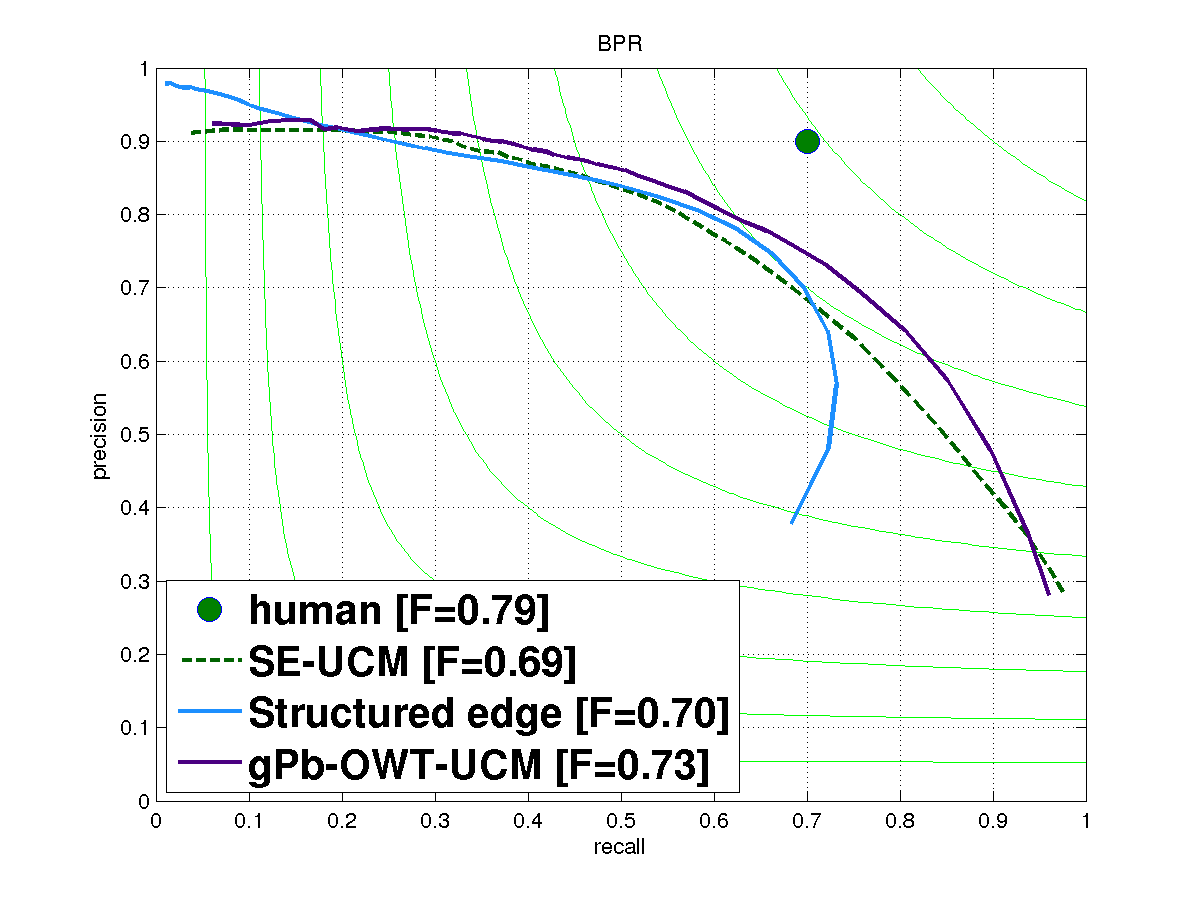
\includegraphics[trim=1.5cm 0cm 1.9cm 0cm, clip=true, width=0.48\textwidth]{images/plots/SE_vs_gPb_OWT_UCM_BPR.png}
 }
 \subfigure[VPR]{%
  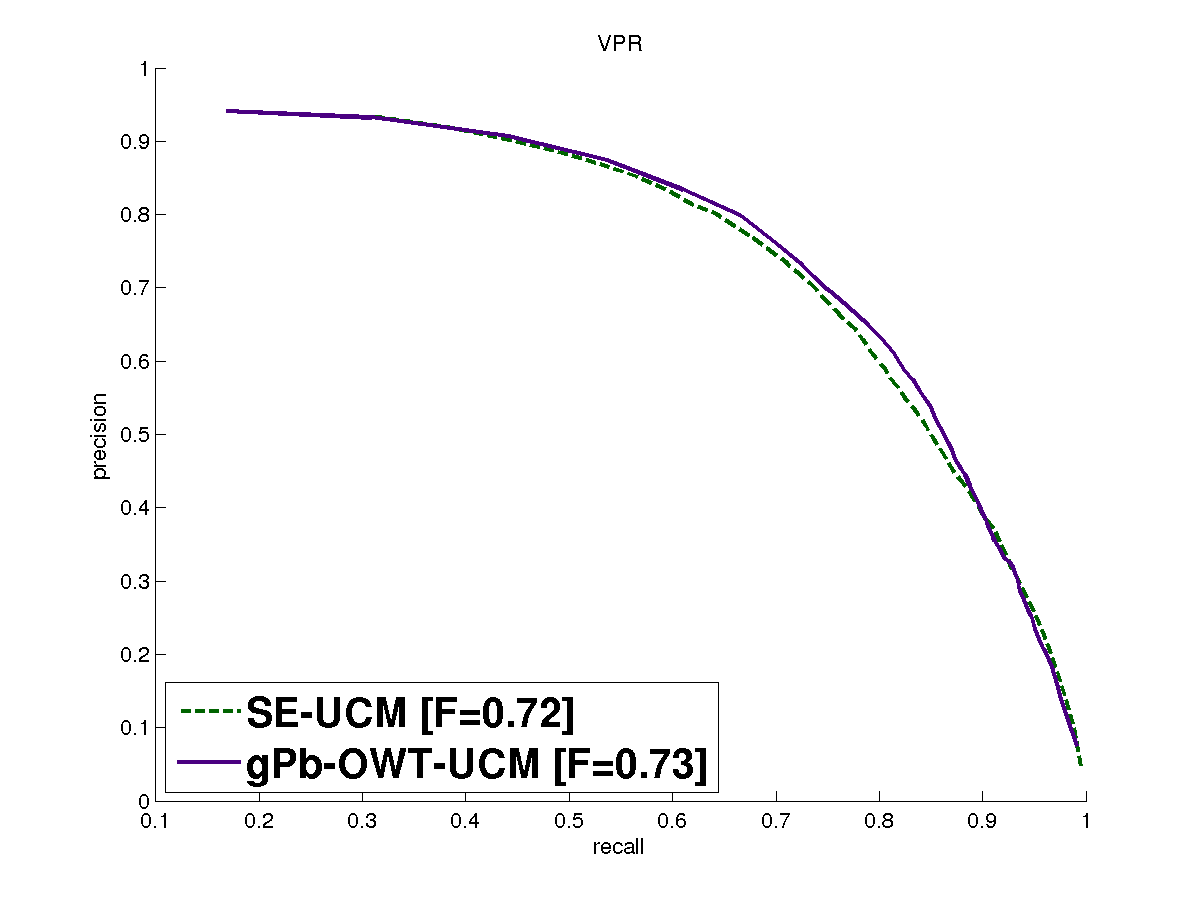
\includegraphics[trim=1.5cm 0cm 1.9cm 0cm, clip=true, width=0.48\textwidth]{images/plots/SE_vs_gPb_OWT_UCM_VPR.png}
 }
\caption[{\tt SE} and {\tt gPb-OWT-UCM} comparison - plots]{We demonstrate the boundary precision recall metric (BPR) and the volume precision recall metric (VPR). Given are the edge detection algorithm that we utilise \textbf{\texttt{SE}}~\cite{DollarICCV13edges} (see the text for parameter details), and the image segmentation algorithm \textbf{\texttt{gPb-OWT-UCM}}~\cite{Arbelaez11}.}
\label{fig:SE_vs_gPb_OWT_UCM}
\end{figure}

\begin{table}[htbp]
\renewcommand{\arraystretch}{1.3}
\centering
\scriptsize
\begin{tabular}{l|c|c|c||c|c|c||c|c|c|}
\cline{2-10} % ZZ
\multirow{2}{*}{} & \multicolumn{3}{c||}{\textbf{BPR}} & \multicolumn{3}{c||}{\textbf{VPR}}& \multicolumn{3}{c|}{\textbf{Region}}\\
\cline{2-10}
& \textbf{ODS}  & \textbf{OIS} & \textbf{AP} % <- BPR
& \textbf{ODS} & \textbf{OSS} & \textbf{AP} % <- VPR
& \textbf{SC} & \textbf{PRI} & \textbf{VoI} \\
\hline
\multicolumn{1}{|l|}{Human} & .79 & .79 & - & - & - & - & .72 & .88 & 1.17 \\ % actually, we had .80 for humans on BPR from \cite{Arbelaez11}; % TODO for VPR - we don't know ODS = OIS for humans
\hline
\hline
\multicolumn{1}{|l|}{\cite{DollarICCV13edges} SE-single} & .70 & .72 & .63 & - & - & - & - & - & - \\
\hline
\multicolumn{1}{|l|}{\cite{Arbelaez11} gPb-OWT-UCM} & .73 & .76 & .77 & .73 & .76 & .78 & .59 & .83 & 1.69 \\
\hline
\end{tabular}
\caption[{\tt SE} and {\tt gPb-OWT-UCM} boundary and region comparison]{{\tt SE} and {\tt gPb-OWT-UCM} boundary and region comparison.}
%The table shows aggregate measures (ODS, OSS, AP) for boundary precision-recall (BPR), volume precision-recall (VPR) and 
%includes region statistics (SC, PRI, VoI).}
\label{tab:SE_vs_gPb_OWT_UCM}
\end{table}

\subsubsection{Benchmark}
We use the benchmark MATLAB code from \cite{Galasso13Benchmark}. %, the metric was introduced in this work~\cite{Galasso13}.
It unifies benchmarks for boundary detection (BPR) and image segmentation (VPR, SC, %ground truth segmentation covering, 
PRI, VoI) and allows the testing of coarse-to-fine methods. %, capturing the trade-off in a precision-recall framework.

\section{From edges to contours - a proof of concept}
\label{sec:ch5-watershed-proof-of-concept}
We apply a {\bf vanilla watershed} algorithm \cite{Beucher1992morphological,Najman1996geodesic,PINKlibrary} to the {\tt SE} output, as described in \sref{sec:ch3-watershed}. The result is a single segmentation. 

In our benchmark plots (\fref{fig:SE-watershed}) the outcome of the experiment is not a Precision-Recall curve, but a single point, %dot, 
indicative of the model error. Since the watershed transformation provides an oversegmentation of the image, the dot is located in the high-recall, low-precision range on the BPR plot (lower right). In contrast, oversegmentations occupy the low-recall, high-precision part of the VPR domain (upper left). 

\begin{figure}[ht!]
\centering
 \subfigure[BPR]{%
  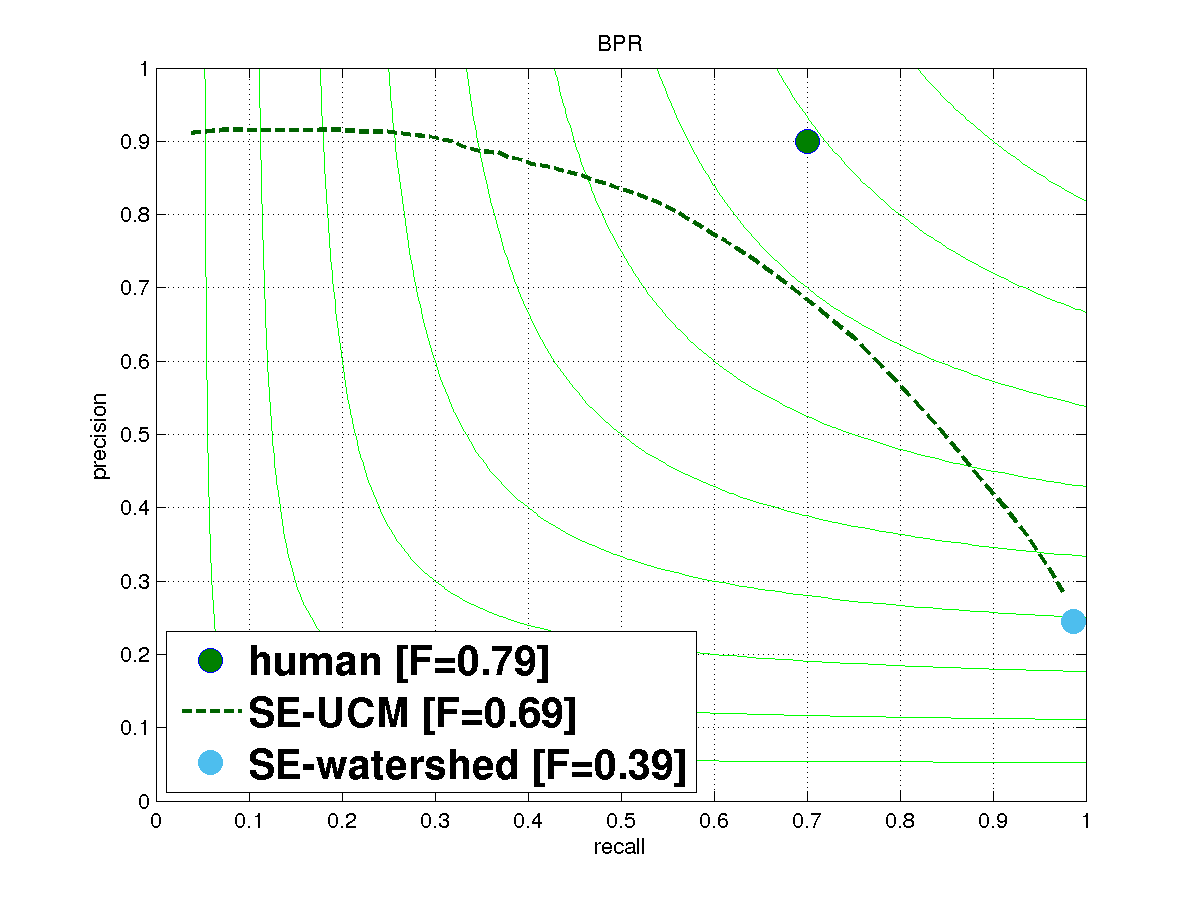
\includegraphics[trim=1.5cm 0cm 1.9cm 0cm, clip=true, width=0.48\textwidth]{images/plots/SE-watershed_BPR.png}
 }
 \subfigure[VPR]{%
  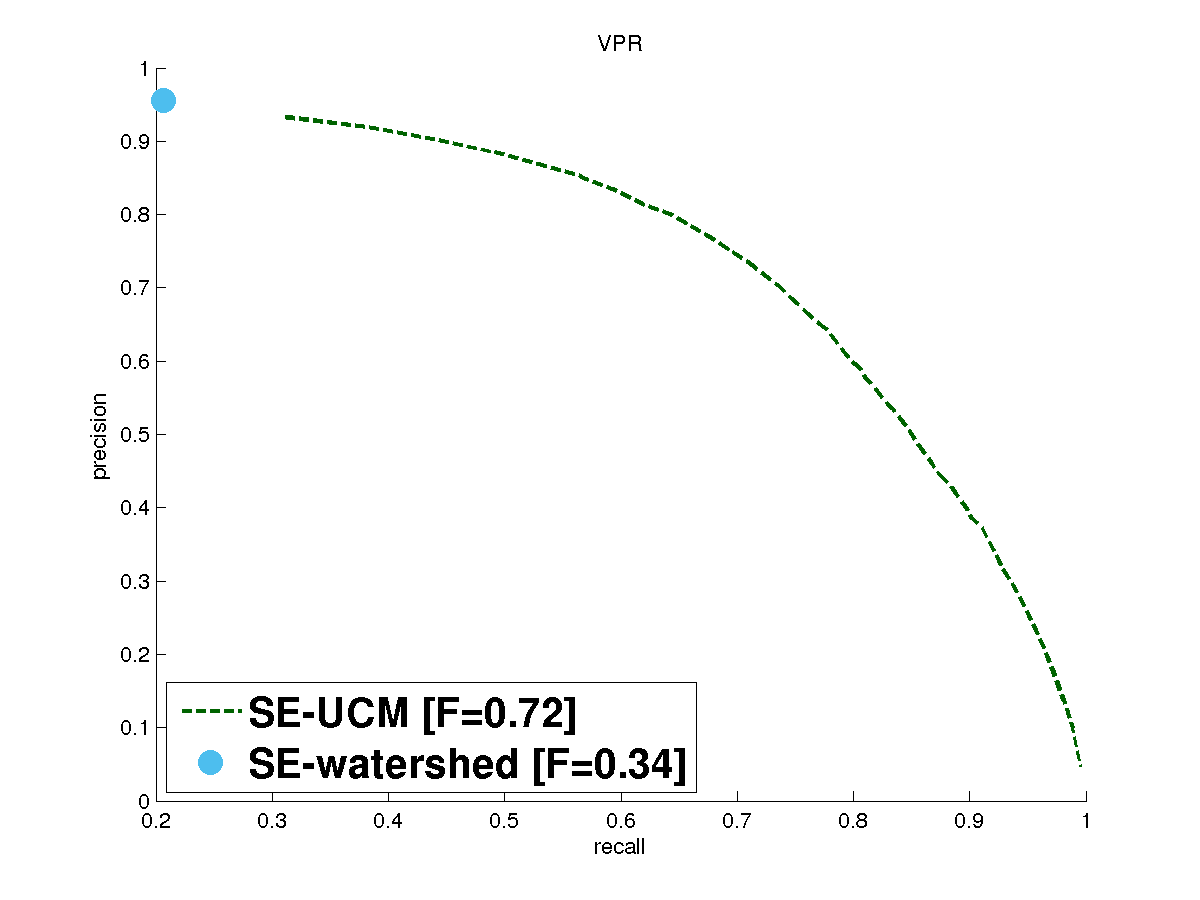
\includegraphics[trim=1.5cm 0cm 1.9cm 0cm, clip=true, width=0.48\textwidth]{images/plots/SE-watershed_VPR.png}
 }
\caption[{\tt SE}-watershed and baseline: {\tt SE-UCM} plots]{\textbf{\texttt{SE}-watershed} (\sref{sec:ch5-watershed-proof-of-concept}) provides a single oversegmentation. Our \textbf{ baseline - \texttt{SE-UCM}} (\sref{sec:ch5-SE-UCM-baseline}) is a {\tt UCM} hierarchy built on top of the probability of boundary output of the {\tt SE} edge detector.}
\label{fig:SE-watershed}
\end{figure}

\subsection{A point at issue % problem, trouble 
with non-maximum suppressed edges}
\label{sec:ch5-nms-issue}
Note that the {\tt SE} algorithm implements non-maximum suppression as a post-processing step on the edge detection output to provide thinned edges. Non-maximum suppression is a method first introduced as a means of reducing thick edge responses to thin lines for the task of edge detection in greyscale images \cite{Rosenfeld1976digital}. Non-maximum suppression considers only the maxima in the gradient direction. As a consequence, the final output of the {\tt SE} often has only a {\bf single regional minimum}. 

When applying the watershed transform in the presence of a {\bf unique lake}, the {\bf watershed is empty}. To circumvent this problem, we use the {\tt SE} detector {\it before non-maxima suppression} as a topographic surface for the flooding.

\section{Baseline: {\tt SE-UCM}}
\label{sec:ch5-SE-UCM-baseline}
As a baseline, we create a hierarchy of segmentations on top of the {\tt SE} detector result. This is in the spirit of \cite{Arbelaez2006boundary} who, however, use the edge detector {\tt Pb} of Martin, Fowlkes and Malik \cite{Martin2004learning}. What we do for this baseline could also be understood %thought 
as our pipeline {\tt SE-SV-UCM} without structured voting ({\tt SV}) at all. Instead, the values from the probability of boundary, which is the output of the edge detector, are directly transferred as values for the watershed contours (effectively performing a ``trivial'' watershed weighting). We then build the multiscale hierarchy - {\tt UCM}. Benchmark plots are on \fref{fig:SE-watershed}.

We observe the problem of strong edges ``bleeding'' into non-salient ones, despite lack of good local boundary evidence, as on the tikis examples (see \fref{fig:SE-UCM-tikis-bleeding-sub2}) between the heads of the middle and right statues. This issue is one of the motivations for the Structured voting (SV) described in \sref{sec:ch4-SE-SV-UCM_SV_details}.% Similarly

\begin{figure}[ht!]
\centering
\subfigure[Input image]{%
 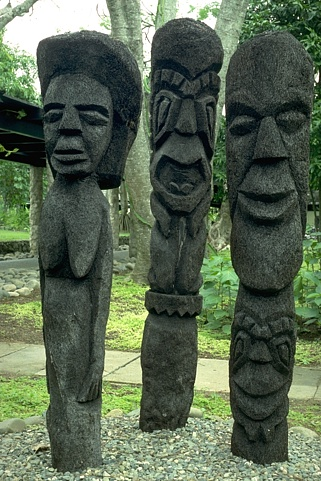
\includegraphics[width=0.32\textwidth]{images/examples/tikis/tikis.jpg}
 \label{fig:SE-UCM-tikis-bleeding-sub1}
}
\subfigure[UCM]{%
 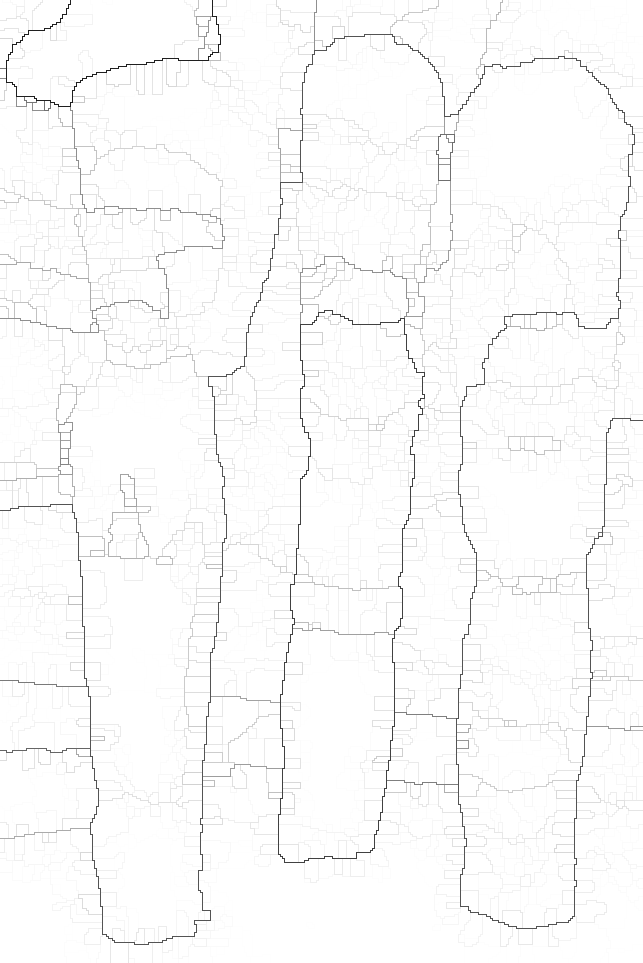
\includegraphics[width=0.32\textwidth,frame]{images/examples/tikis/SE-UCM-tikis-ucm-problem.png}
 \label{fig:SE-UCM-tikis-bleeding-sub2}
}
\caption[{\tt SE-UCM} drawback - ``bleeding'' of strong edges towards unimportant ones]{\textbf{\texttt{SE-UCM}} result. \protect\subref{fig:SE-UCM-tikis-bleeding-sub1} - an image from the validation subset of \cite{BSDS500resources}. Notice how in the {\tt SE-UCM} output \protect\subref{fig:SE-UCM-tikis-bleeding-sub2} unimportant horizontal edges between the statues' heads are {\it incorrectly %wrongly 
up-voted} due to strong vertical boundary in their vicinity (the outline of the statues).}
\label{fig:SE-UCM-tikis-bleeding}
\end{figure}
% BPR edge detector Pb (previously ``MFM'') Pb 0.65, Pb-UCM 0.67
% SE 0.70, % SE_no_nms_single_scale_repeat
% SE-UCM 0.69 (0.70)

\section{{\tt (SE+sPb)-OWT-UCM}}
\label{sec:ch5-SE_sPb-OWT-UCM}
{\tt (SE+sPb)-OWT-UCM} is a modification of {\tt gPb-OWT-UCM} that we described in \cref{Chapter3}, where we replace the edge detector {\tt mPb} and use {\tt SE} instead (see \fref{fig:SE_sPb-OWT-UCM-details-SE_sPb_gPb}). Unlike the original method, we don't use multiscale information.

\begin{figure}[ht!]
\centering
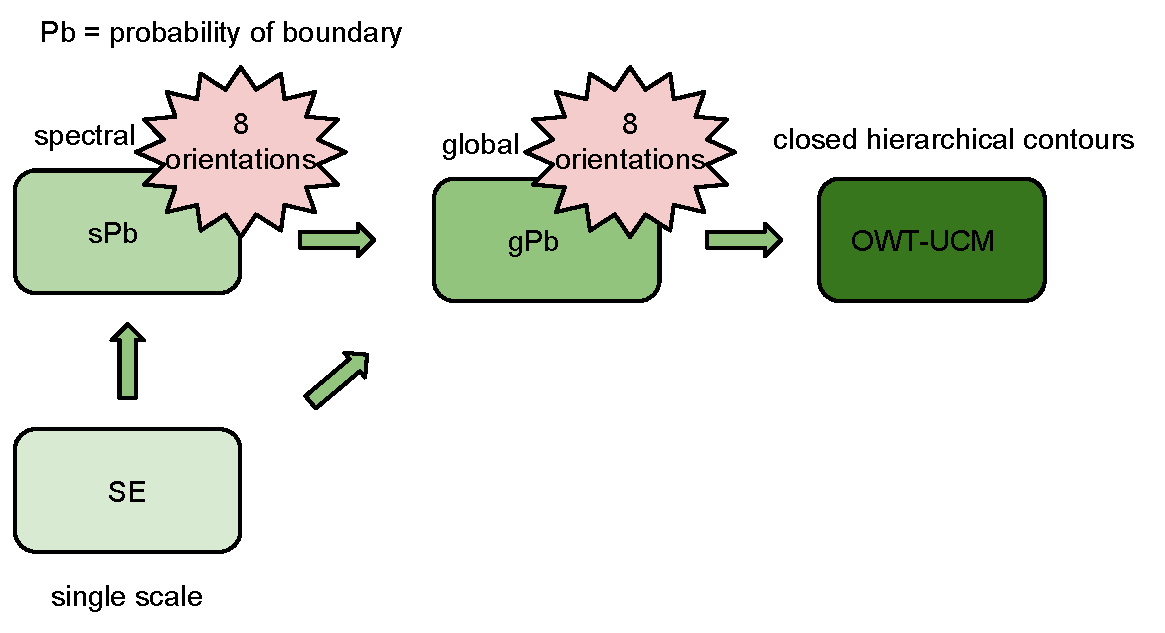
\includegraphics[width=1\textwidth]{images/experiments/SE_sPb-OWT-UCM/SE_sPb-OWT-UCM-details-SE_sPb_gPb.pdf}
\caption[{\tt (SE+sPb)-OWT-UCM} pipeline with focus on the edge-detection stage]{We replace the {\tt gPb} edge detector in {\tt gPb-OWT-UCM} with {\tt SE}. Compare to the detailed {\tt gPb-OWT-UCM} from \fref{fig:gPb-algorithm-details-mPb_sPb_gPb}.}
\label{fig:SE_sPb-OWT-UCM-details-SE_sPb_gPb}
\end{figure}


% NOTE the following was wrong
% {\tt (SE+sPb)-OWT-UCM} is an improvement of the baseline \sref{sec:ch5-SE-UCM-baseline}, where we enhance the edge detector and again proceed to directly copy the detector values to the watershed contours (effectively performing a ``trivial'' watershed weighting). We then build the multiscale hierarchy - {\tt UCM}. 

\textbf{Our method permits to introduce globalisation:} This experiment shows us that {\bf globalisation could easily be introduced} to our method. Here we use the same affinity matrix as the spectral detector {\tt sPb} and weighted combination to obtain {\tt gPb} of Arbel\'aez \etal \cite{Arbelaez11}. Extending our algorithm to adopt such a globalisation step could be beneficial, since it would be able to pick up on improvements in the realm of {\it spectral partitioning}, as for example spectral reduction \cite{Galasso14}. % check the plots, check MCG paper - they did exactly this

\textbf{Spectral partitioning leads to higher precision:} Edge detection methods employing spectral clustering % partitioning have been reported to do 
work well in the high-precision, low-recall regime of BPR and are comparatively weaker in the low-precision, high-recall regime \cite{Fowlkes04,Yu2005segmentation}. We already performed similar reasoning when comparing {\tt mPb} and {\tt sPb} in Section~\ref*{sec:ch3-Pb_mPb_sPb_gPb}~\ref{par:ch3-Pb_mPb_sPb_gPb}. 
Hence, it is not surprising to see in \fref{fig:SE_nnms_sPb-UCM_BPR} the shift, compared to {\tt SE-OWT}, of the {\tt (SE+sPb)-OWT-UCM} curve towards better precision {\bf at the expense of recall}.

\textbf{Multiscale techniques %allow to 
discover more edges:} Comparing {\tt (SE+sPb)-OWT-UCM} to {\tt gPb-OWT-UCM} in \fref{fig:SE_nnms_sPb-UCM_BPR} shows us that segmentation using {\tt gPb} is superior in the high-recall regime. This is due to {\tt mPb} being employed at the edge-discovering stage, see \sref{sec:ch3-mPb}. This is also clear to see in the visual comparison of the edges extracted by the two methods in \fref{fig:SE_sPb-OWT-UCM-visual}.

The VPR only manifests barely perceptible differences %improvement 
between the three methods 
- see \fref{fig:SE_nnms_sPb-UCM_VPR}.

\begin{figure}[ht!]
\centering
 \subfigure[BPR]{%
  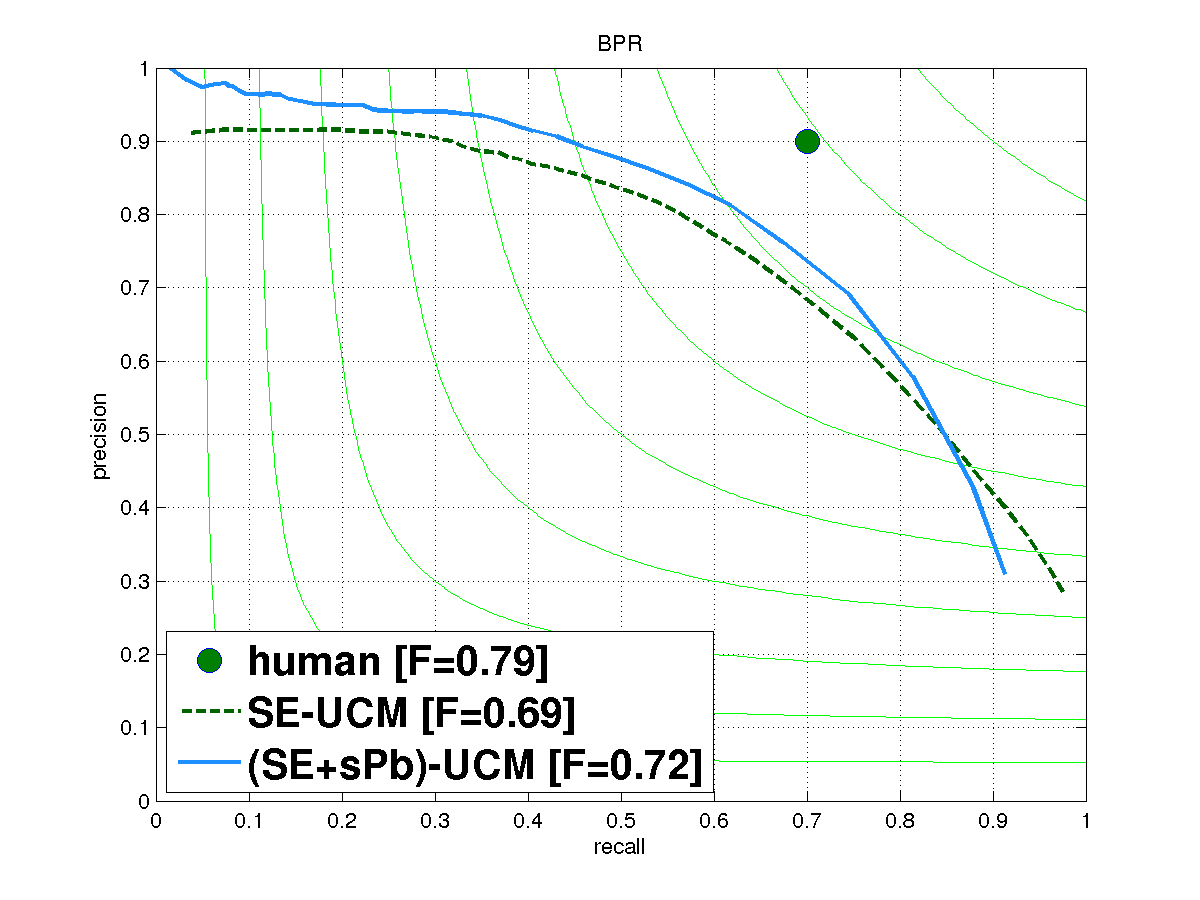
\includegraphics[trim=1.5cm 0cm 1.9cm 0cm, clip=true, width=0.48\textwidth]{images/plots/SE_nnms_sPb-UCM_BPR.png}
  \label{fig:SE_nnms_sPb-UCM_BPR}
 }
 \subfigure[VPR]{%
  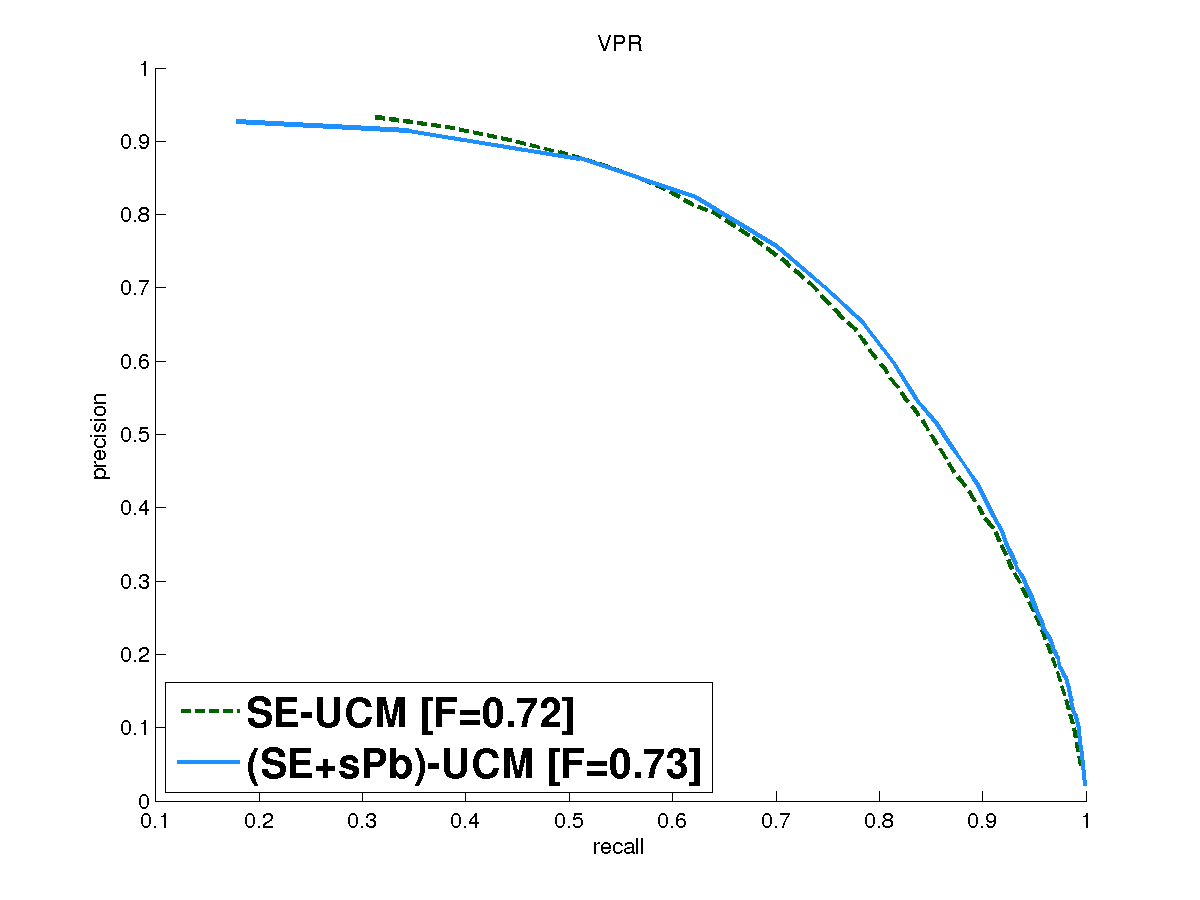
\includegraphics[trim=1.5cm 0cm 1.9cm 0cm, clip=true, width=0.48\textwidth]{images/plots/SE_nnms_sPb-UCM_VPR.png}
  \label{fig:SE_nnms_sPb-UCM_VPR}
 }
\caption[{\tt (SE+sPb)-OWT-UCM} plots]{{\tt (SE+sPb)-OWT-UCM} results confirm that spectral methods help %mostly 
discover more salient edges - improved precision and slight decline in recall on the BPR metric. See the text for details.}
\label{fig:SE_nnms_sPb-UCM}
\end{figure}

\begin{figure}[ht!]
\begin{center}
  \begin{tabular}{ c c c }
  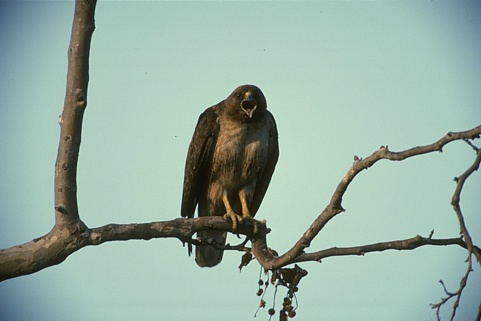
\includegraphics[width=0.3\textwidth]{images/experiments/SE_sPb-OWT-UCM/eagle.png} &
  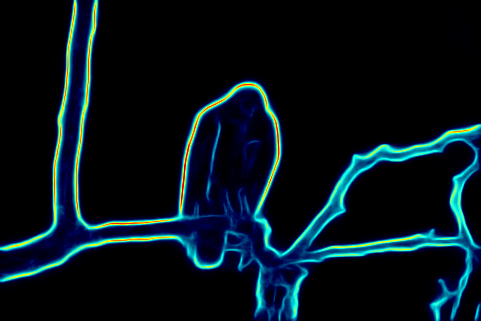
\includegraphics[width=0.3\textwidth]{images/experiments/SE_sPb-OWT-UCM/eagle_SE-UCM_Pb_not_nms.png} &
  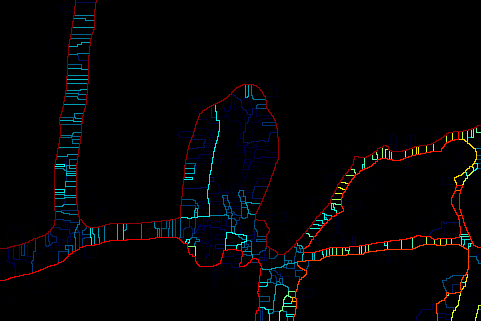
\includegraphics[width=0.3\textwidth]{images/experiments/SE_sPb-OWT-UCM/eagle_SE-UCM_ucm_imageSize.png} \\
  &
  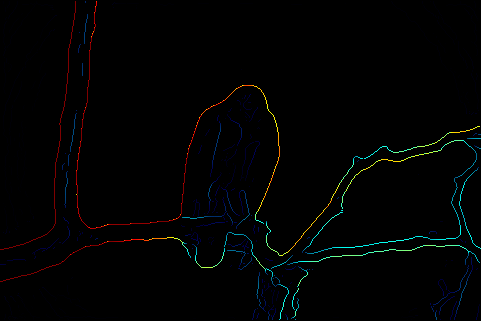
\includegraphics[width=0.3\textwidth]{images/experiments/SE_sPb-OWT-UCM/eagle_gPb-OWT-UCM_gPb_thin.png} &
  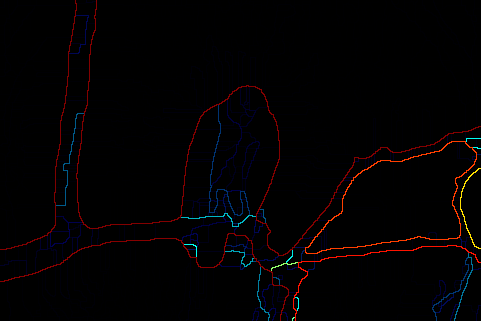
\includegraphics[width=0.3\textwidth]{images/experiments/SE_sPb-OWT-UCM/eagle_gPb-OWT-UCM_ucm_imageSize.png} \\
  &
  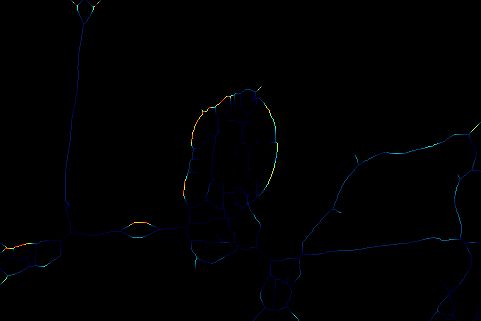
\includegraphics[width=0.3\textwidth]{images/experiments/SE_sPb-OWT-UCM/eagle_(SE_sPb)-OWT-UCM_gPb_thin.png} &
  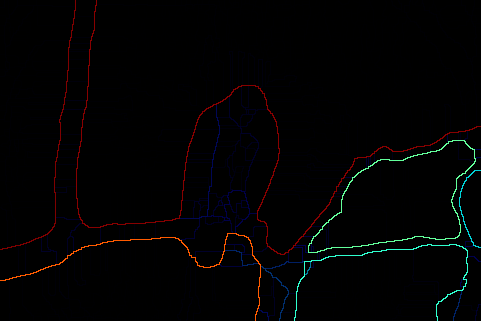
\includegraphics[width=0.3\textwidth]{images/experiments/SE_sPb-OWT-UCM/eagle_(SE_sPb)-OWT-UCM_ucm_imageSize.png} \\
  Input image & Pb (\ie, edges) & {\tt UCM} (\ie, segmentation) \\
  \end{tabular}
\end{center}
\caption[{\tt SE-UCM}, {\tt gPb-OWT-UCM} and {\tt (SE+sPb)-OWT-UCM} - a visual comparison]{A visual comparison of the methods evaluated in \fref{fig:SE_nnms_sPb-UCM}. {\bf First row}: {\tt SE-UCM} (notice that the edges must not be thinned, as \sref{sec:ch5-nms-issue} argues), {\bf second row}: {\tt gPb-OWT-UCM} and {\bf third row}: {\tt (SE+sPb)-OWT-UCM}.}
\label{fig:SE_sPb-OWT-UCM-visual}
\end{figure}


\section[Structured voting]{Structured voting - experimental study of watershed weighting strategies} % Weighting strategies % Exploration of the Space of Weighting Strategies
\label{sec:ch5-structured-voting}
All experiments presented here are instances of the general algorithm described in \sref{sec:ch4-SE-SV-UCM_SV_details}. Each of them implements the SV differently, \ie, in the following we offer a systematic exploration of the space of watershed weighting strategies.

\subsection{Superpixels and Rand index}
We leave the watershed patch to be an oversegmentation, which in fact it is. The output of the watershed transform that we use has {\bf explicit} the boundaries between segments, which would hinder a region-based metric. Therefore, we transform a watershed patch to have {\bf implicit segment boundaries} - the locations of transition between differently labelled segments. See \sref{sec:ch1-segmentation-terminology} for the definitions and \fref{fig:sub:segmentation-segm-labelling} for examples of the two types of segmentation representation. With a representation as a {\bf segmentation labelling} we can use a region-based metric for the patches comparison.

The patches from the decision forest already constitute segmentation labelling with implicit segment boundaries. That, of course, is due to the fact that the structured forest patches are taken unmodified from the ground truth segmentations of the training subset of BSDS500, which has a ``labelling with implicit segment boundaries'' format (see \fref{fig:BSDS-annotations}). 

We conduct the comparison between watershed and a tree leaf patch using as a scoring function one of:

\begin{enumerate}
 \item{\bf Rand Index (RI):} a count of the number of pairs of locations that belong to the same segment in both patches. For a $16\times16$ segmentation patch, that means $32 640$ pairs of locations. Section~\ref*{sec:ch4-boundary-and-region-metrics-maths}~\ref{par:ch4-RI-maths} contains the formula of the RI.
 \item{\bf Rand Index Monte Carlo (RIMC):} ours randomised subsample version of RI, which takes only a fraction $\rho$ of the pairs of locations into consideration. We defined %mathematically 
 the metric in Section~\ref*{sec:ch4-boundary-and-region-metrics-maths}~\ref{par:ch4-RIMC-maths}. We experience no reduction in performance \wrt RI for a fraction as small as $\rho\approx\frac{1}{128}$, \ie, 256 out of the $32 640$ possible pairs of locations in a $16 \times 16$ patch. This scoring function is inspired from the way features are subsampled to introduce randomness when training a decision tree in~\cite{DollarICCV13edges,Dollar2013toolbox}.
\end{enumerate}

The above experiments (both having a result of $F=0.55$ on BPR) led us to two conclusions. First, we need to have a closer look into the properties of our \textbf{scoring functions}. Section~\ref{sec:ch4-boundary-and-region-metrics-maths} of the previous chapter gives mathematical formulae and a detailed explanation on the metrics we considered for this task. Second, a \textbf{simplification of the watershed patch} is desirable, due to the discrepancy %mismatch between 
in makeup %constitution
of watershed and decision tree patches.

\subsection{Na\"{\i}ve greedy merge of watershed patch}
We first address the second of our conclusions from the previous experiment. We merge segments in the watershed patch according to each of the $T$ leaf patches (where $T$ is the number of trees in the decision forest). Thus we end up with $T$ distinct ``merged'' watershed patches. This approach seems to be too greedy, however. The watershed patch eventually becomes overly adapted to the tree leaf patch it is being compared to. As a consequence, this watershed transformation is not discriminative enough.

\subsubsection{Fair greedy merge}
To remedy this shortcoming of the na\"{\i}ve greedy merge, we introduce what we call ``fairness'' in the greedy merge approach. As described previously, we cast votes only on the watershed locations. That means, the patches that we consider contain a potential boundary location at their central pixel. It is the strength of this boundary that we strive to quantify. We enforce the greedy merge to respect a boundary-at-centre-location condition by preventing excessive merge of the segments around the central pixel of the patch.

\begin{figure}[ht!]
\centering
 \subfigure[Input image]{%
  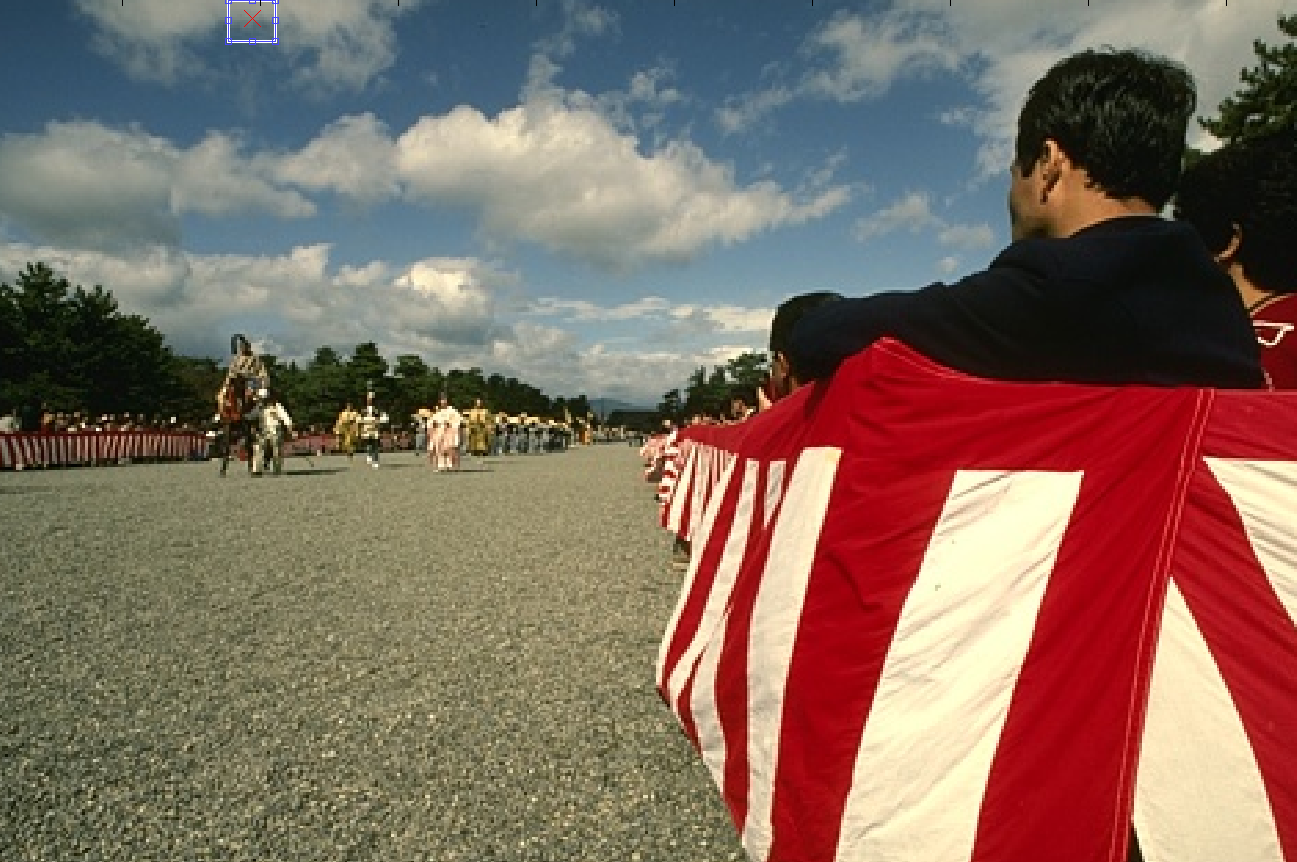
\includegraphics[width=0.5\textwidth]{images/experiments/ws-greedy-merge/corrida.png}
 }
 \subfigure[Cropped image patch]{%
  
\includegraphics[width=0.2\textwidth]{images/experiments/ws-greedy-merge/selected-image-patch.png}
 }

 \subfigure[Cropped watershed patch]{%
  
\includegraphics[width=0.2\textwidth,frame]{images/experiments/ws-greedy-merge/watershed-colour-coded.png}
  %\label{fig:sub:ws-greedy-merge-ws-colour-coded}
 }
 \subfigure[Watershed patch with implicit region boundaries]{%
  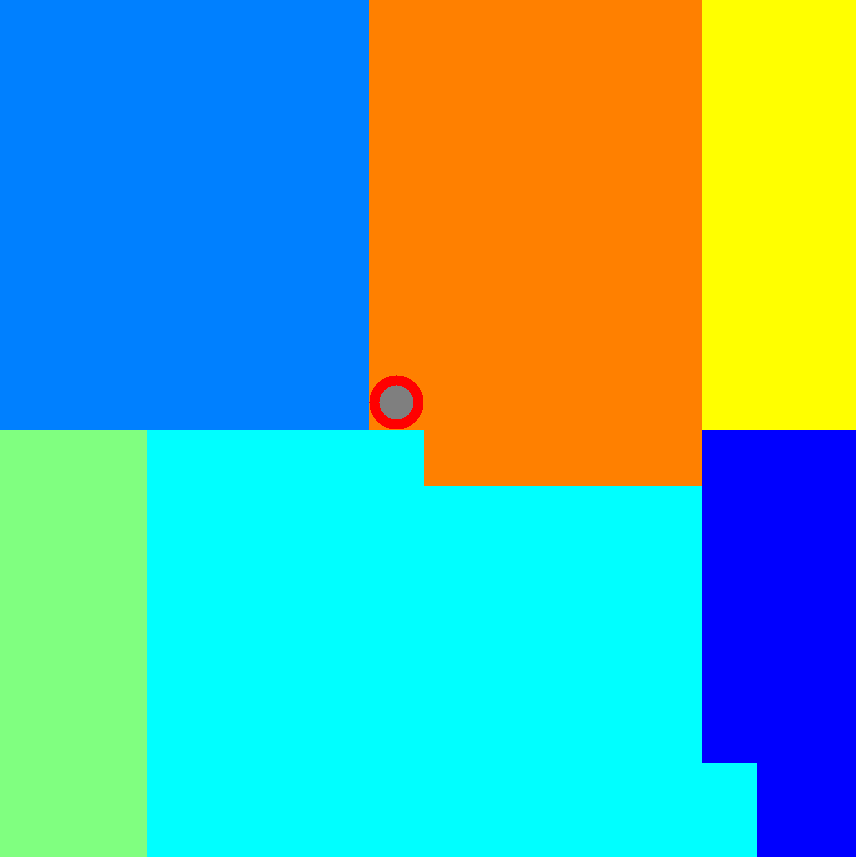
\includegraphics[width=0.2\textwidth,frame]{images/experiments/ws-greedy-merge/watershed-segments.png}
  %label{fig:sub:ws-greedy-merge-ws-segments}
 } \qquad\qquad\qquad\qquad\qquad

 \subfigure[Tree leaf segmentation patch that guides the merging]{%
  \fboxrule=2pt %border thickness
  \fcolorbox{red}{white}{\fboxrule=0.5pt 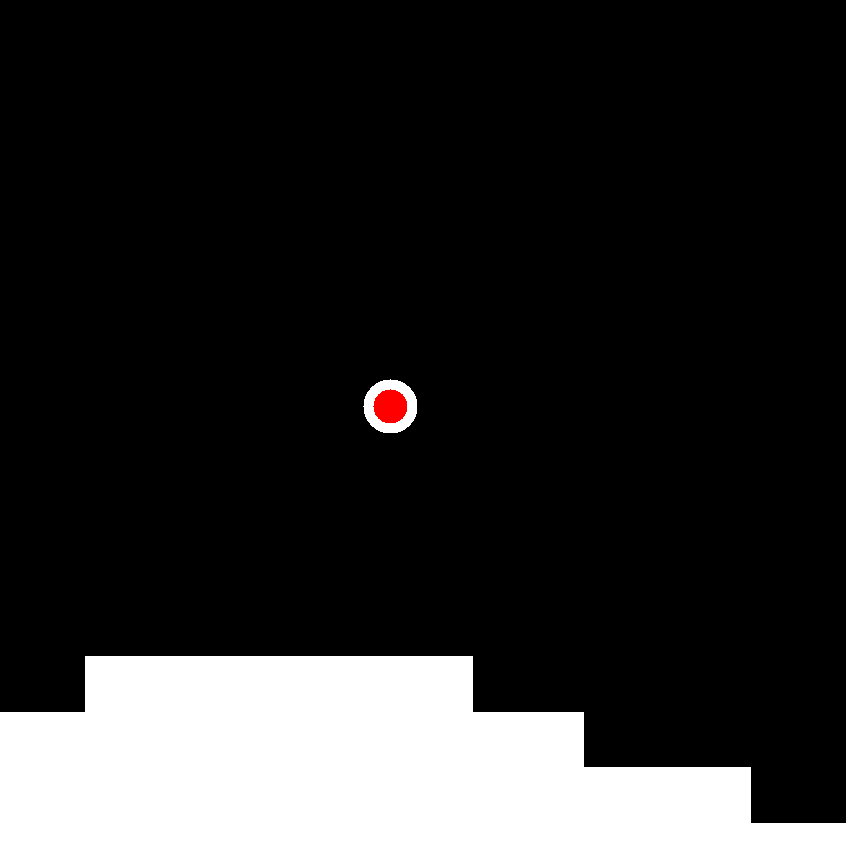
\includegraphics[width=0.2\textwidth,frame]{images/experiments/ws-greedy-merge/tree-leaf.png}}
  \label{fig:sub:ex-ws-greedy-merge-tree-leaf}
 }
 \subfigure[Watershed patch {\bf na\"{\i}ve} greedy merge]{%
  
\includegraphics[width=0.2\textwidth,frame]{images/experiments/ws-greedy-merge/watershed-naive-greedy-merge.png}
  \label{fig:sub:ex-ws-greedy-merge-ws-naive-greedy-merge}
 }
 \subfigure[Watershed patch {\bf fair} greedy merge]{%
  \fboxrule=2pt %border thickness
  \fcolorbox{green}{white}{\fboxrule=0.5pt 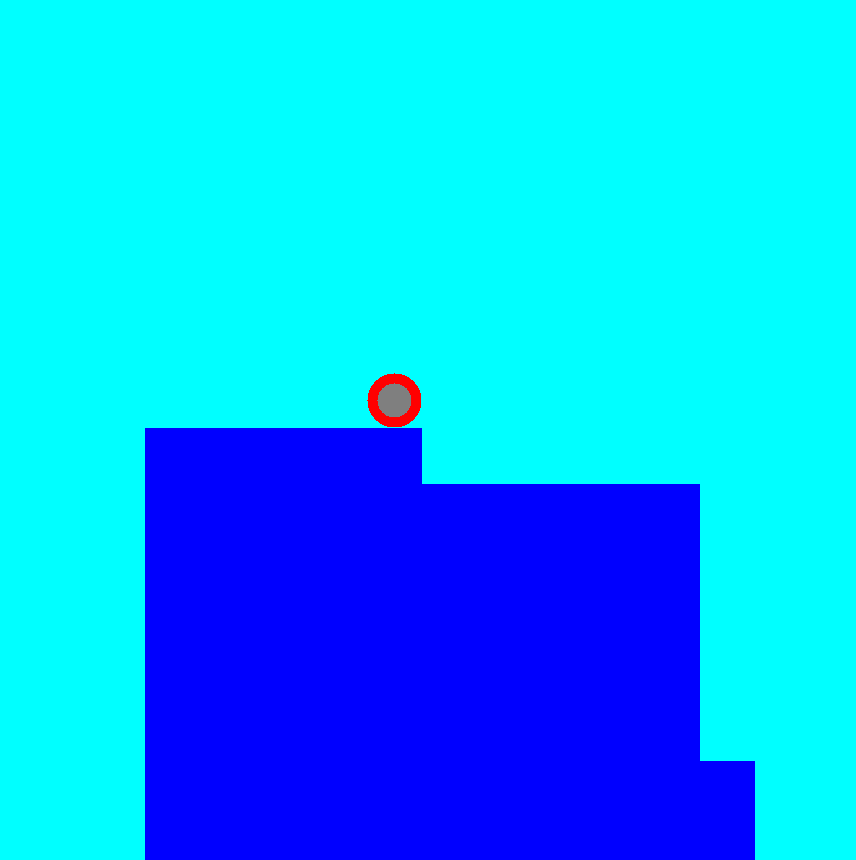
\includegraphics[width=0.2\textwidth,frame]{images/experiments/ws-greedy-merge/watershed-fairer-greedy-merge.png}}
  \label{fig:sub:ex-ws-greedy-merge-ws-fairer-greedy-merge}
 }
\caption[{\bf Greedy merge} of watershed patch.]{{\bf Greedy merge} of watershed patch. The central pixel of the patches is marked, as it is important, see the text for details. The comparison is between a tree leaf patch (in red \protect\subref{fig:sub:ex-ws-greedy-merge-tree-leaf}) and a watershed patch (in green \protect\subref{fig:sub:ex-ws-greedy-merge-ws-fairer-greedy-merge}).}
\label{fig:ex-ws-greedy-merge} % experiments-ws-greedy-merge
\end{figure}

\fref{fig:segs-to-greedy-merge-RIMC} shows the improvement we get over watershed oversegmentation with the last two experiments.

\begin{figure}[ht!]
\centering
 \subfigure[BPR]{%
  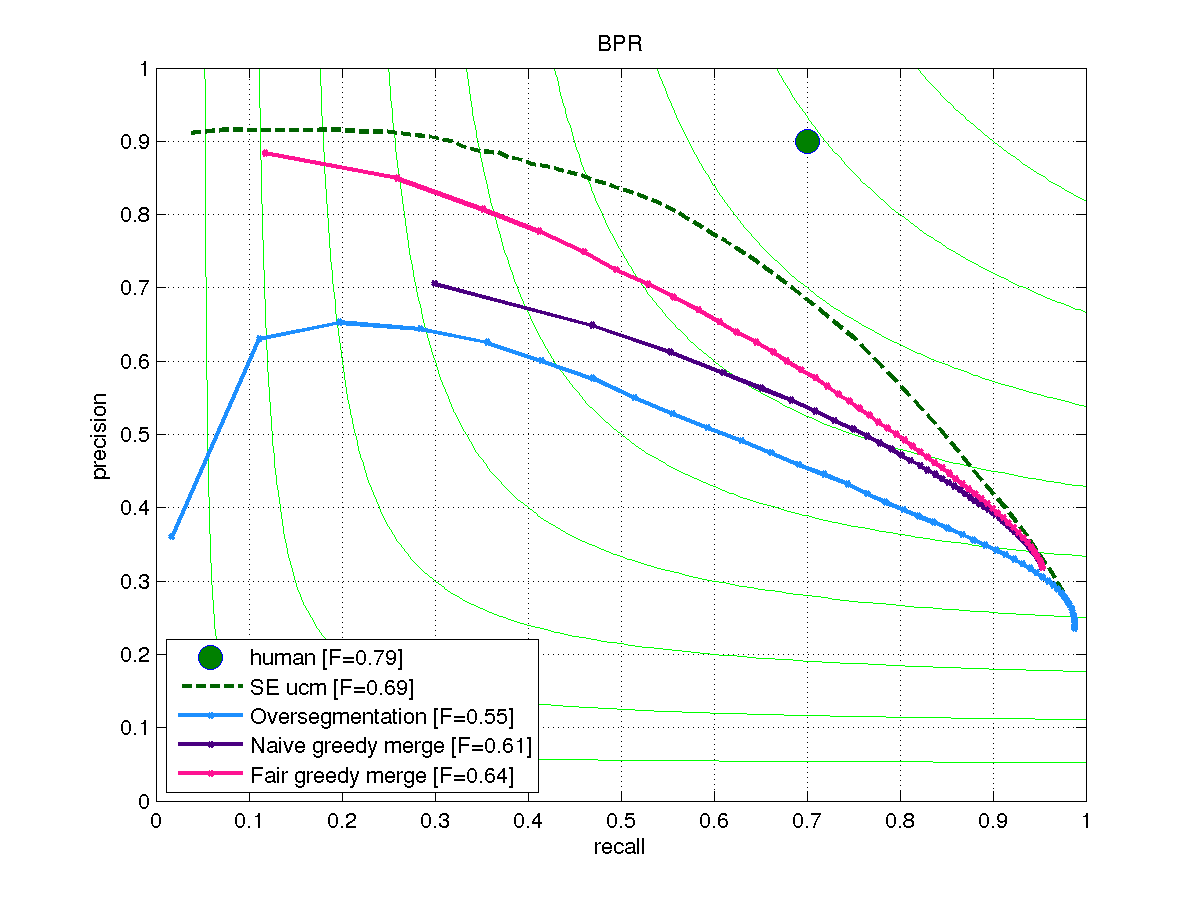
\includegraphics[trim=1.5cm 0cm 1.9cm 0cm, clip=true, width=0.48\textwidth]{images/plots/segs-to-greedy-merge-RIMC-BPR.png}
 }
 \subfigure[VPR]{%
  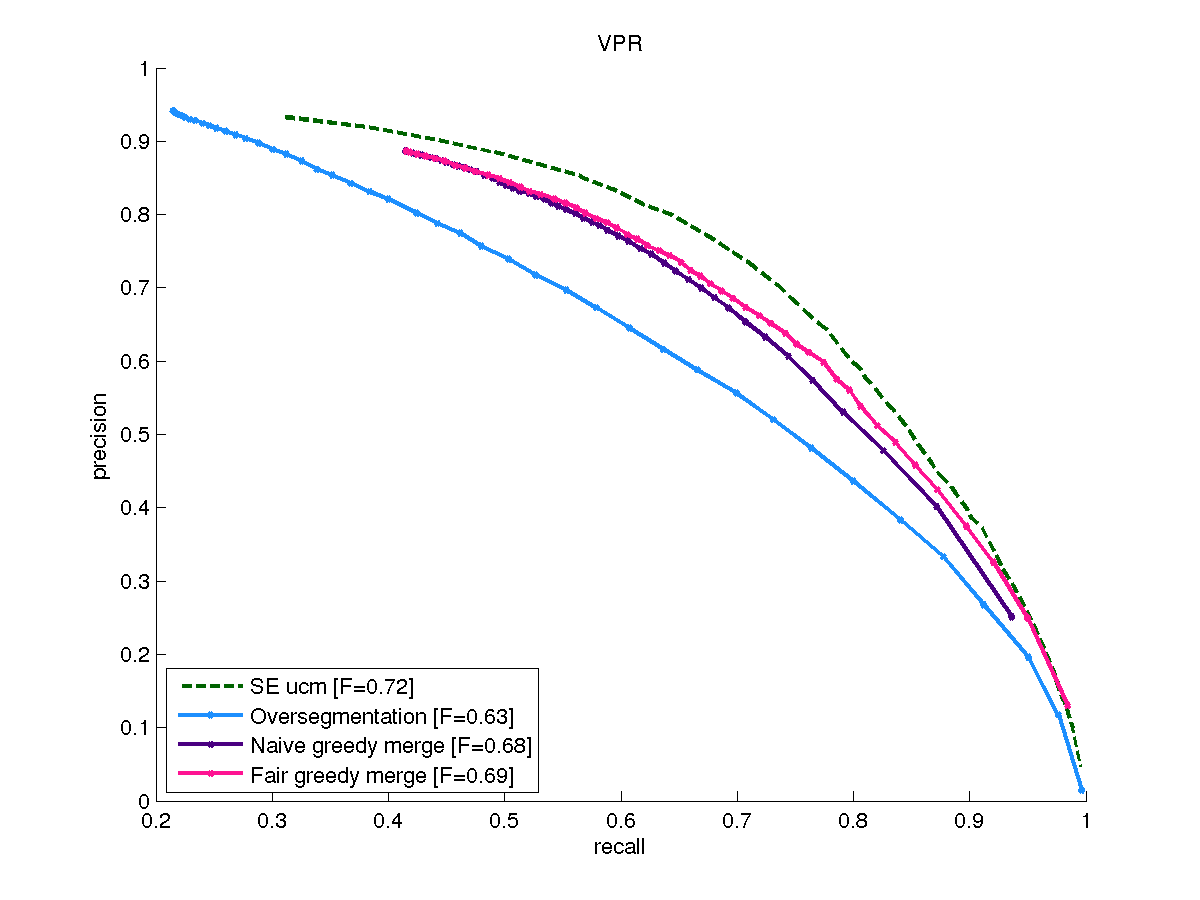
\includegraphics[trim=1.5cm 0cm 1.9cm 0cm, clip=true, width=0.48\textwidth]{images/plots/segs-to-greedy-merge-RIMC-VPR.png}
 }
\caption[Greedy merge experiments - plots]{Greedy merge experiments. In all cases the scoring function used for patches comparison was the RIMC (Section~\ref*{sec:ch4-boundary-and-region-metrics-maths}~\ref{par:ch4-RIMC-maths} contains a description of the RIMC metric).} % (\hyperref[par:ch4-RIMC-maths]{RIMC description in Chapter 4}).} % that looks bad on paper, still useful for .pdf, as it contains the link
\label{fig:segs-to-greedy-merge-RIMC}
\end{figure}

\subsection{Line fitting}
This is our best performing weighting strategy. As we explained in Section~\ref*{sec:ch4-patch-transformations}~\ref{par:ch4-line-fitting}, we implemented three slightly different line fitting algorithms:
\begin{enumerate}
  \item parametric, based on the derivative direction of the {\bf end-points} of the watershed arc we vote on,
  \item as above, but enforcing adherence to the {\bf centre pixel} of the image patch,
  \item {\bf linear least squares} fitting (LLS) to all the watershed arc pixels.
 % also possible - PCA-based fit
\end{enumerate}

\tref{tab:line-fitting-experiments} summarises performance results from the line fitting methods \wrt different scoring functions. For brevity, we only included % report
the ODS F-measure of the BPR metric and remark, that the BPR and VPR curves, as well as the region metrics confirm the ranking of the experiments. 
It is notable that all 3 types of scoring functions - VPR, RI, BPR perform reasonably well with this watershed transformation. We include results for the two types of normalisation for VPR - on the side of the watershed, and on the side of the tree leaf patch.

% TODO prettify (make the cells equally big); UPDATE with new results
\begin{table}[htbp]
\renewcommand{\arraystretch}{1.3}
\centering
\scriptsize
% \begin{tabular}{|l||c|c|c||c|c|c||c|c|c||}
\begin{tabular}{|l|c|c|c|c|}
\hline 
Line fitting method & VPR (watershed) & VPR (trees) & RI & BPR \\
\hline 
% \hline 
end vertices & {\bf .69} & {\bf .63} & {\bf .68} & {\bf .67} \\
patch centre & {\bf .69} & {\bf .63} & {\bf .68} & .66 \\
LLS & .68 & {\bf .63} & {\bf .68} & .66 \\
\hline
\end{tabular}
\caption[Our three types of line fitting results summary]{Our three types of line fitting results summary. For each method we have tried all our scoring functions. See the text for details.}
\label{tab:line-fitting-experiments}
\end{table}

% Discuss performance \wrt different scoring functions. Notable that all 3 types of scoring functions - VPR, RI, BPR perform reasonably well with this watershed transformation. Normalisation of VPR. Asymmetry of normalisation and how it affects us.

\subsection{Watershed arc}
We would like our watershed weighting strategy to take into account fine changes in the shape of the region boundary. To this end, we transform the watershed patch to contain exclusively the part of the watershed on which we are to cast our vote - the recursively subdivided {\bf watershed arc}, and discard all other (parts of) region boundaries present in the patch, as we described in Section~\ref*{sec:ch4-patch-transformations}~\ref{par:ch4-watershed-arc}.

This approach does not guarantee closed contours - the part of the region boundary present in the patch would often be {\bf just an image edge}. So we cannot use as a scoring function a region metric but must instead use a boundary-based one. We must, therefore, transform the segmentation patch from the tree leaf to a boundary patch. It is easy to obtain an edge map, given a segmentation (see details in \sref{sec:ch1-segmentation-terminology}). Our transformed tree leaf patch is a binary edge map. As a scoring function we use the boundary-based evaluation metric - {\bf BPR} (see Section~\ref*{sec:ch4-boundary-and-region-metrics-maths}~\ref{par:ch4-BPR-maths}).

\fref{fig:watershed-arc-experiment} utilises the same scoring function - BPR, to allow for the fair comparison of two patch transformations: the watershed arc which we described here and the line fitting from the previous sections' set of experiments. 

Our conclusion from this experiment is that the combination of only the edge with the BPR provides poor means of judging the evidence of boundary in the leaves of the structured forest. Watershed arc is a very brittle cue per se. % intrinsically, in itself

Further, as we explained in Section~\ref*{sec:ch4-boundary-and-region-metrics-maths}~\ref{par:ch4-BPR-maths}, BPR is parametrised on the pixel distance threshold for which a match between the two segmentation boundaries is to be made. While for natural images a value of 3 or 4 pixels works fine, this parameter is a bit of an issue for small local patches of size $16\times 16$. There is no generic way to correctly choose such a distance for all pairs of a forest segmentation patch and a watershed contours patch. Accurate localisation of boundaries seems to be crucial for this weighting strategy, and this is not the case with the leaf segmentations and the watershed.

\begin{figure}[ht!]
\centering
 \subfigure[BPR]{%
  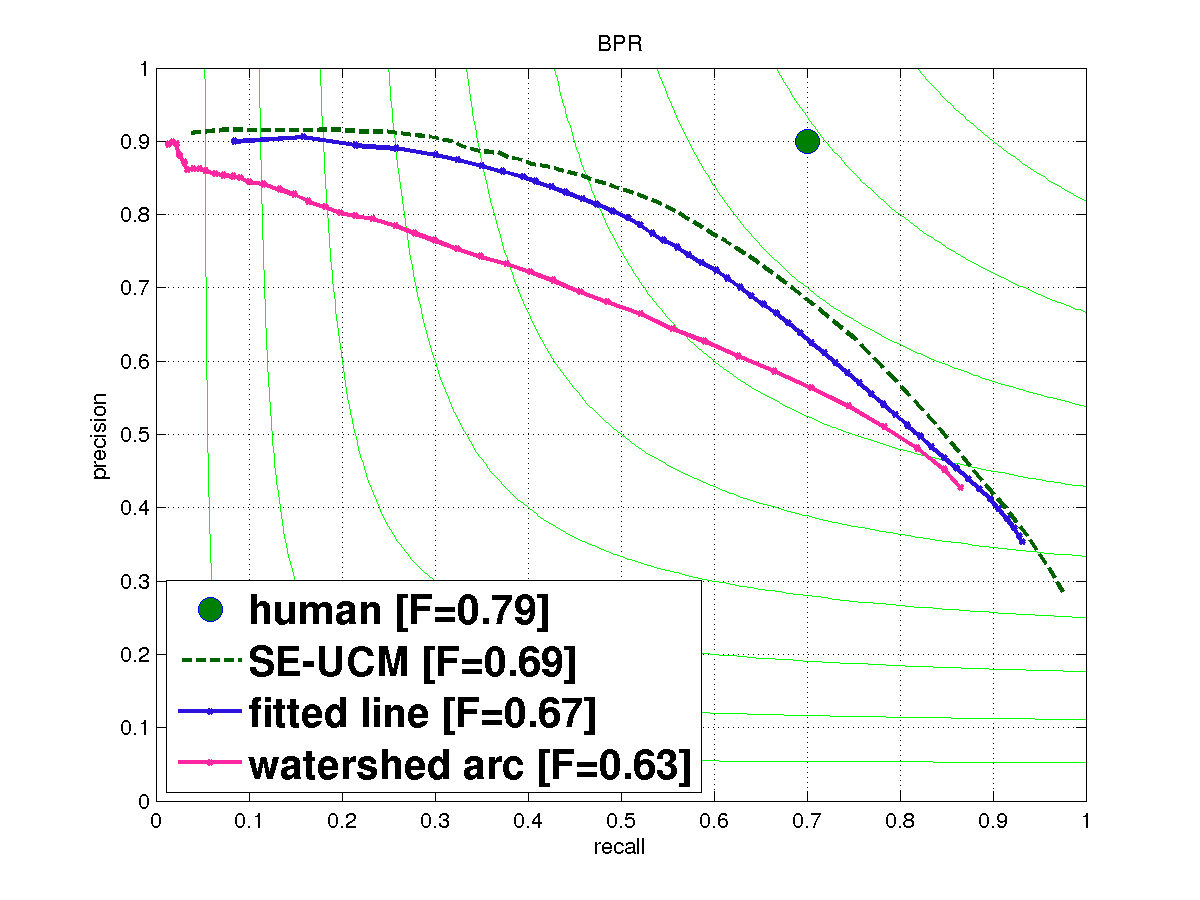
\includegraphics[trim=1.5cm 0cm 1.9cm 0cm, clip=true, width=0.48\textwidth]{images/plots/watershed-arc-experiment_BPR.png}
 }
 \subfigure[VPR]{%
  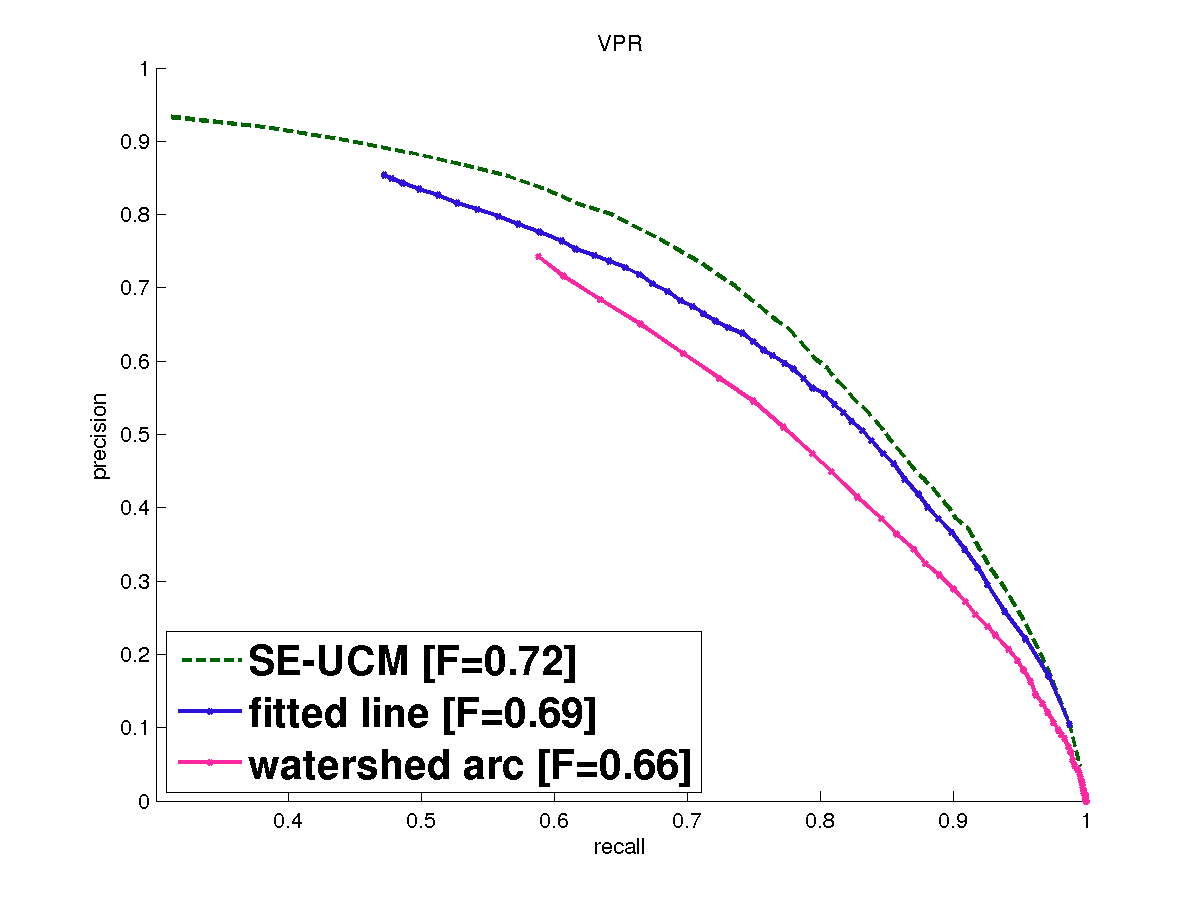
\includegraphics[trim=1.5cm 0cm 1.9cm 0cm, clip=true, width=0.48\textwidth]{images/plots/watershed-arc-experiment_VPR.png}
 }
\caption[{\bf Watershed arc} compared to fitting a line as a patch transformation - plots]{{\bf Watershed arc} compared to fitting a line through the end points of the watershed arc as a patch transformation. The scoring function for the two experiments was the BPR metric with a distance threshold for the bipartite matching = 3 pixels.}
\label{fig:watershed-arc-experiment}
\end{figure}

\subsection{Quadratic fitting} % conic n=2; Polynomial
This experiment implements the patch transformation described in Section~\ref*{sec:ch4-patch-transformations}~\ref{par:ch4-quadratic-lls-fitting}. This richer model allows not only for fitting a {\bf line}, but also for any of the 3 conic sections - a {\bf parabola}, a {\bf hyperbola}, or an {\bf ellipse}, to explain the data. See \fref{fig:ws-quadratic-fitting} for a few examples of the thus transformed watershed patches.

As discussed in Section~\ref*{sec:ch4-patch-transformations}~\ref{par:ch4-quadratic-lls-fitting}, this seems to be too complex a model, thwarted by degenerate cases. At times the best fitting parameters would yield a 3-dimensional surface that only just misses to intersect the patch plane, % $Z=0$ plane
leading to an empty patch as the solution for a transformed watershed.

In \fref{fig:quadratic-lls-fitting} and \tref{tab:quadratic-lls-fitting} we show the results of comparing the two linear least squares (LLS) approaches - the {\bf linear} vs. the {\bf quadratic} one. The missing recall in \fref{fig:quadratic-lls-fitting-BPR}, respectively, missing precision in \fref{fig:quadratic-lls-fitting-VPR} for the quadratic model indicates that the method has a tendency to {\bf undersegment}. 
Indeed, \fref{fig:quadratic-lls-fitting-visual} confirms this, additionally offering a visual comparison of the outputs of the two algorithms. The quadratic model performs poorly and leads to pronounced {\bf artefacts} where small closed contours are chosen above long extended ones. Notice how VPR \fref{fig:quadratic-lls-fitting-VPR} and the region metrics in \tref{tab:quadratic-lls-fitting} much better reflect the supremacy of the simpler linear model to the quadratic one. % superiority

\begin{figure}[ht!]
\centering
 \subfigure[BPR]{%
  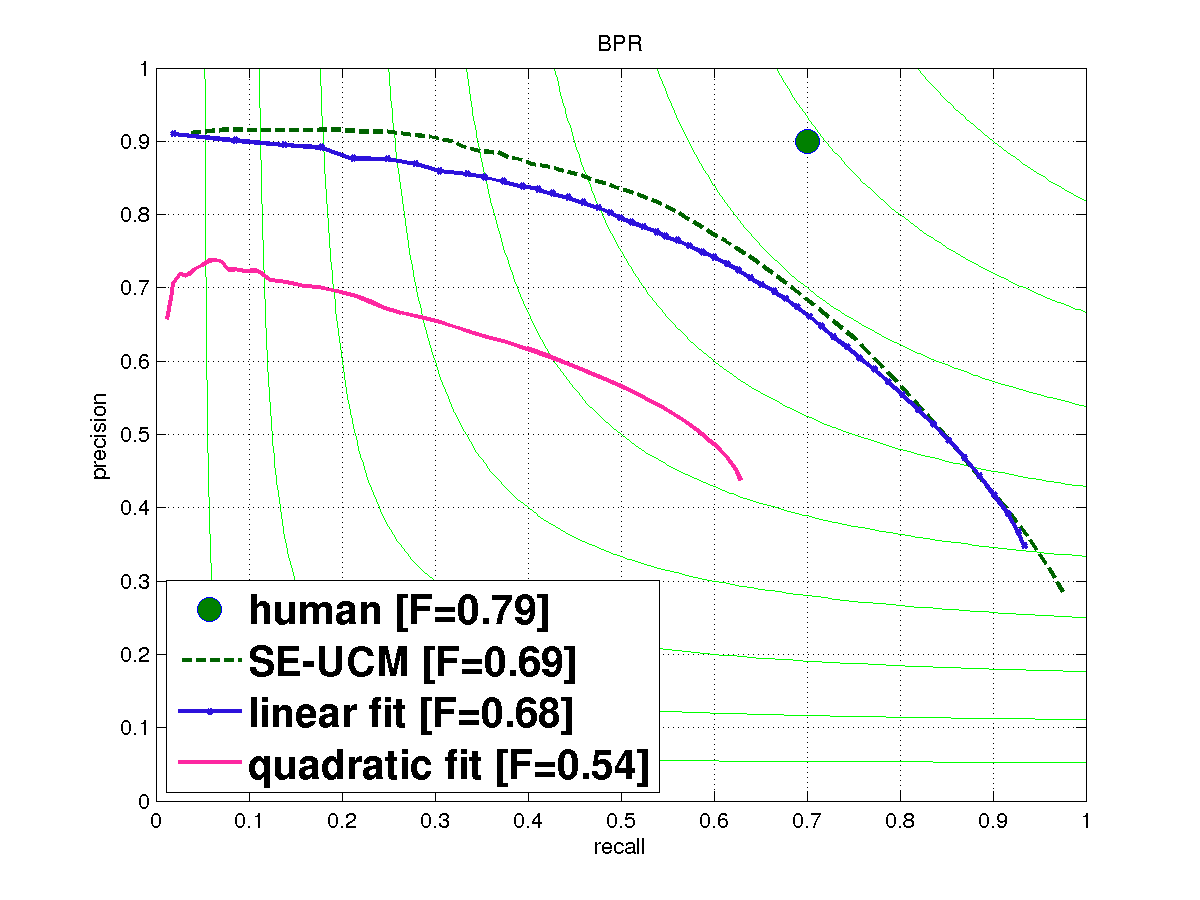
\includegraphics[trim=1.5cm 0cm 1.9cm 0cm, clip=true, width=0.48\textwidth]{images/plots/SE-quadratic_BPR.png}
  \label{fig:quadratic-lls-fitting-BPR}
 }
 \subfigure[VPR]{%
  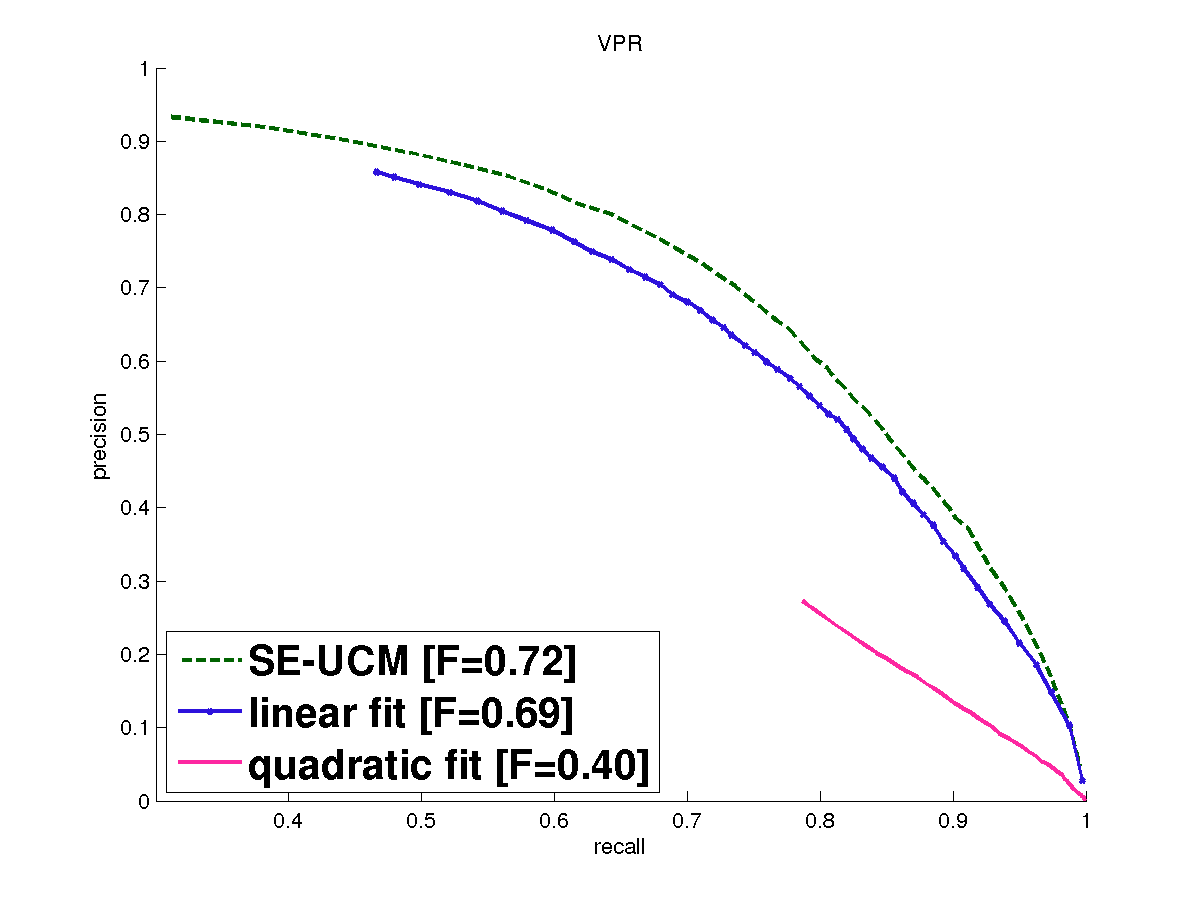
\includegraphics[trim=1.5cm 0cm 1.9cm 0cm, clip=true, width=0.48\textwidth]{images/plots/SE-quadratic_VPR.png}
  \label{fig:quadratic-lls-fitting-VPR}
 }
\caption[{\bf Quadratic} linear least squares fitting compared to the {\bf linear} model - plots]{{\bf Quadratic} linear least squares fitting compared to the {\bf linear} model. The scoring function for the two experiments was the VPR normalised on the side of the watershed.}
\label{fig:quadratic-lls-fitting}
\end{figure}

\begin{table}[htbp]
\renewcommand{\arraystretch}{1.3}
\centering
\scriptsize
\begin{tabular}{l|c|c|c||c|c|c||c|c|c|}
\cline{2-10} % ZZ
\multirow{2}{*}{} & \multicolumn{3}{c||}{\textbf{BPR}} & \multicolumn{3}{c||}{\textbf{VPR}}& \multicolumn{3}{c|}{\textbf{Region}}\\
\cline{2-10}
& \textbf{ODS}  & \textbf{OIS} & \textbf{AP} % <- BPR
& \textbf{ODS} & \textbf{OSS} & \textbf{AP} % <- VPR
& \textbf{SC} & \textbf{PRI} & \textbf{VoI} \\
\hline
\multicolumn{1}{|l|}{linear LLS} & .68 & .71 & .71 & .69 & .71 & .71 & .55 & .81 & 1.90 \\% linear model - linear least squares fitting}
\hline
\multicolumn{1}{|l|}{quadratic LLS} & .54 & .56 & .40 & .40 & .40 & .25 & .37 & .55 & 2.45 \\
\hline
\end{tabular}
\caption[{\bf Quadratic} linear least squares fitting compared to the {\bf linear} model - table]{{\bf Quadratic} linear least squares fitting compared to the {\bf linear} model - benchmark scores on BSDS500~\cite{BSDS500resources}.}
\label{tab:quadratic-lls-fitting}
\end{table}

\begin{figure}[ht!]
\centering
 \subfigure[Input image]{%
  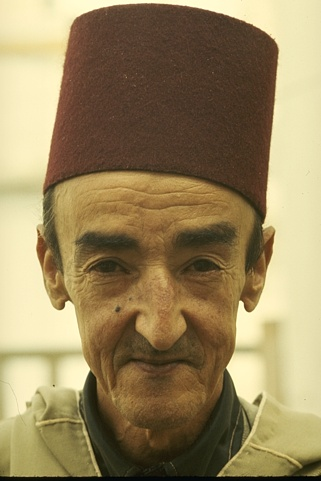
\includegraphics[width=0.31\textwidth]{images/experiments/quadratic-lls/old_man_input.png}
 }
 \subfigure[Linear LLS]{%
  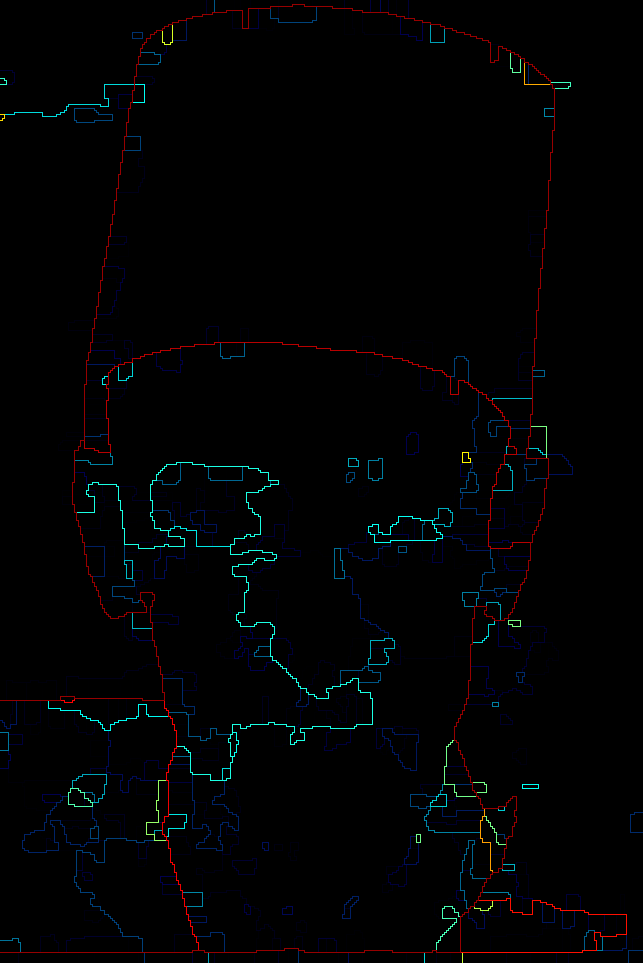
\includegraphics[width=0.31\textwidth]{images/experiments/quadratic-lls/old_man_UCM_line_lls_VPR_normalised_ws.png}
 }
 \subfigure[Quadratic LLS]{%
  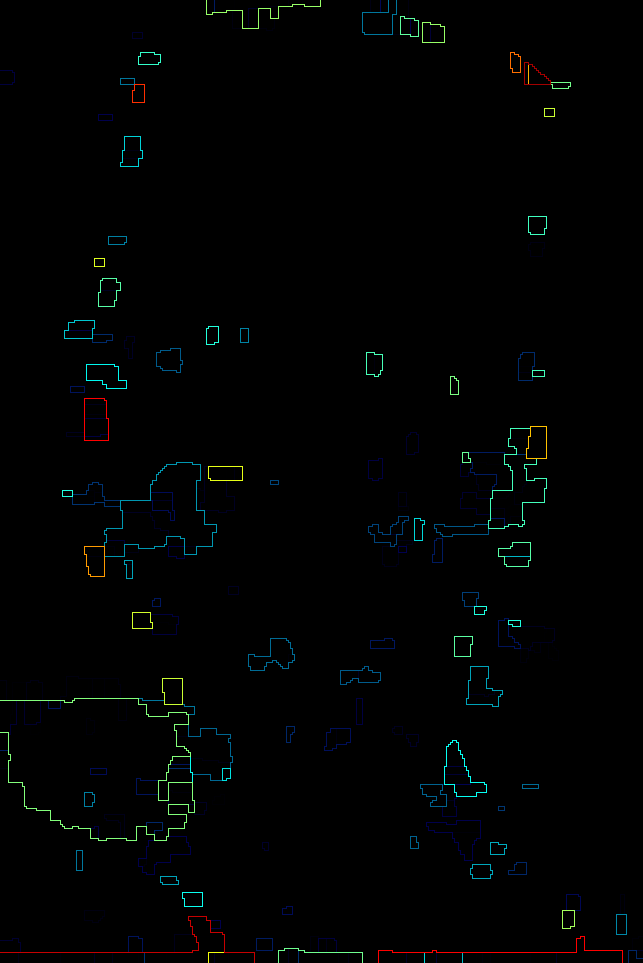
\includegraphics[width=0.31\textwidth]{images/experiments/quadratic-lls/old_man_UCM_conic_VPR_normalised_ws.png}
 }
\caption[{\bf Quadratic} linear least squares fitting compared to the {\bf linear} model - output]{{\bf Quadratic} linear least squares fitting compared to the {\bf linear} model. The quadratic model is much more conservative in casting a vote, and although it fires near salient edges, it displays a tendency towards small, jagged closed segments.}
\label{fig:quadratic-lls-fitting-visual}
\end{figure}

\section[Oracle for Structured voting]{Oracle for Structured voting - experiments using ground truth}
\label{sec:ch5-oracle}
To evaluate the correctness of our weighting strategies, we've implemented an oracle for our pipeline. The question we wanted to answer is ``how well could we perform segmentation in the presence of perfect information?'' Our Structured voting (SV) lends itself easily to such an experiment using the ground truth segmentation. 

\subsection{Oracle definition}
For the oracle, just like in the regular experiments (in \sref{sec:ch5-structured-voting}), when scoring a given pixel on the watershed regions boundary, one of the patches is cropped centred around that same pixel location in the watershed contours image. The second patch, as we alluded %to 
in \sref{sec:ch4-asymmetry-VPR-assigning-patches-S-G} when discussing argument assignment for asymmetric metrics, is a ground truth segmentation patch. This is different from SV (\sref{sec:ch5-structured-voting}), which uses the trained model - the inferred most likely segmentation learnt by the structured forest.

% oracle - experiments with the ground truth 4 methods + 4 corresponding oracles
% (a). quadratic LLS + VPR normalised on the side of the watershed
% (b). fairer greedy merge + VPR normalised on the side of the trees
% (c). watershed arc + BPR 3
% (d). line (ends) + RI

\subsection{Compared weighting strategies}
We have chosen to compare here 4 methods and their corresponding oracles. \fref{fig:oracle} contains their precision-recall quantitative results. Each method uses a different {\bf patch transformation} and a different {\bf scoring function} than the others: 
\begin{enumerate}
 \item[(a)] quadratic LLS fitting (Section~\ref*{sec:ch4-patch-transformations}~\ref{par:ch4-quadratic-lls-fitting}) + VPR normalised on the side of the watershed (Section~\ref*{sec:ch4-boundary-and-region-metrics-maths}~\ref{par:ch4-VPR-maths}),
 \item[(b)] fairer greedy merge (Section~\ref*{sec:ch4-patch-transformations}~\ref{par:ch4-fair-greedy-merge}) + VPR normalised on the side of the trees (Section~\ref*{sec:ch4-boundary-and-region-metrics-maths}~\ref{par:ch4-VPR-maths}),
 \item[(c)] watershed arc (Section~\ref*{sec:ch4-patch-transformations}~\ref{par:ch4-watershed-arc}) + BPR (Section~\ref*{sec:ch4-boundary-and-region-metrics-maths}~\ref{par:ch4-RI-maths}), and 
 \item[(d)] %parametric 
 fitted line through the end vertices of the watershed arc (Section~\ref*{sec:ch4-patch-transformations}~\ref{par:ch4-line-ends}) + RI (Section~\ref*{sec:ch4-boundary-and-region-metrics-maths}~\ref{par:ch4-RI-maths}).
\end{enumerate}

\begin{figure}[ht!]
\centering
 \subfigure[BPR]{%
  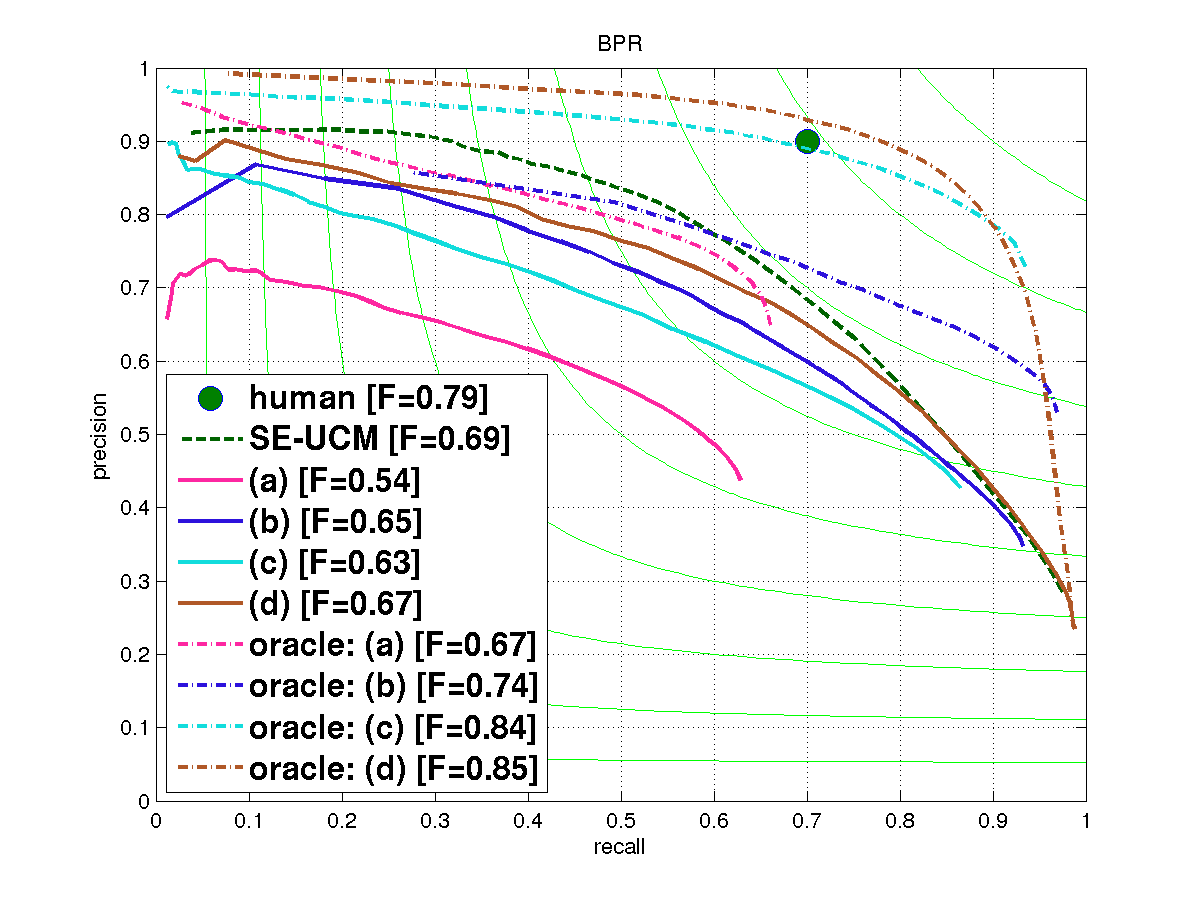
\includegraphics[trim=1.5cm 0cm 1.9cm 0cm, clip=true, width=0.48\textwidth]{images/plots/oracle_BPR.png}
 }
 \subfigure[VPR]{%
  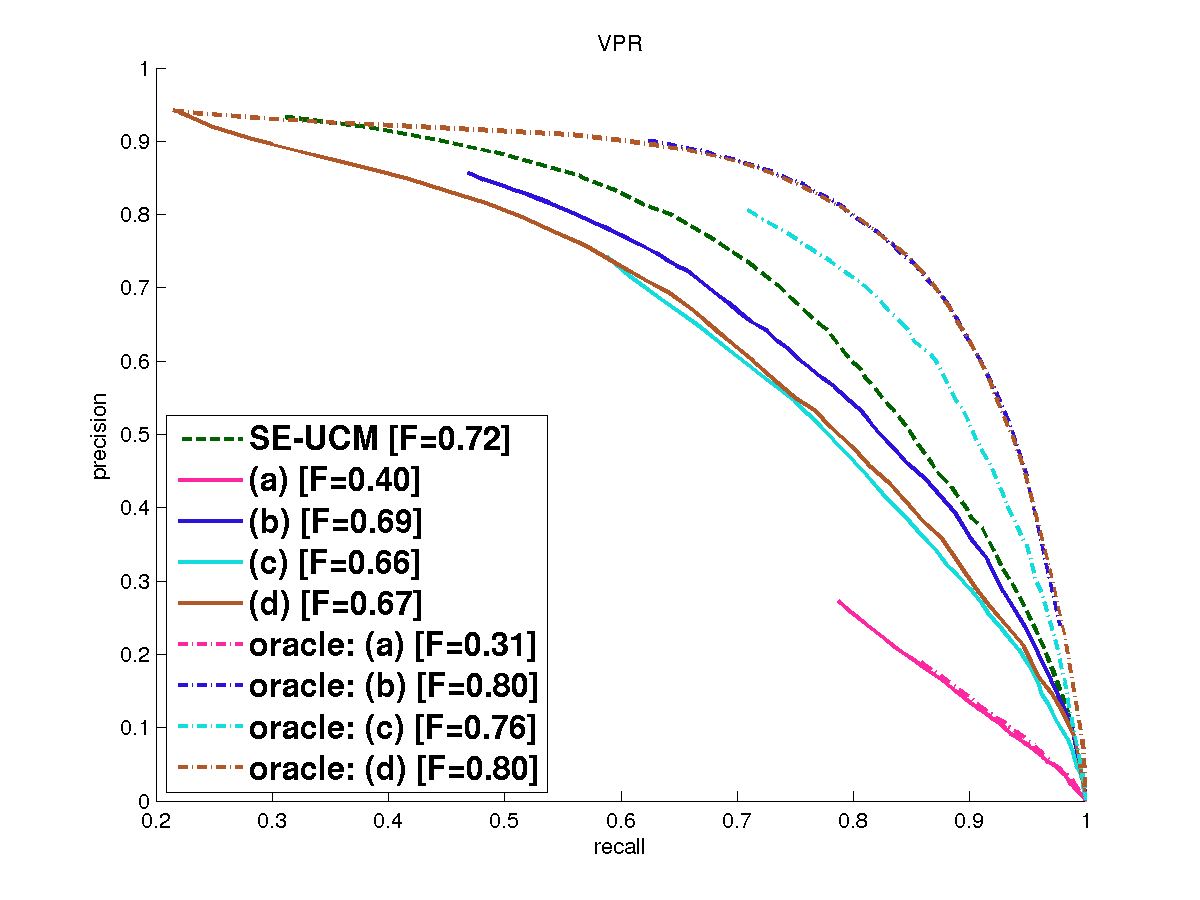
\includegraphics[trim=1.5cm 0cm 1.9cm 0cm, clip=true, width=0.48\textwidth]{images/plots/oracle_VPR.png}
 }
\caption[Oracle experiments using the ground truth - plots]{Oracle experiments using the ground truth. See the text for the details on the methods and analysis.}
\label{fig:oracle}
\end{figure}

% Ranking of oracles confirms Correct Weighting Strategies % NOTE not quite :)
\subsection{Conclusions of the oracle experiments}
\begin{enumerate}
 \item a weak patch transformation as the quadratic LLS fitting cannot be helped even by a good scoring function {\bf (a)}. Since this SV is very conservative and only finds a few edges, there is a lot of lost recall in the BPR metric. The VPR, however, provides a more realistic evaluation. The fact that the presence of perfect leaf information does not improve the segmentation shows us that this is quite poor way of closing edge into contours.
 \item we consider the rest of the methods - {\bf (b), (c), (d)} to be valid, successful ways of obtaining hierarchical segmentations. All of them do benefit from the improved comparison with the ground truth (and not the SF leaves). Both in BPR and VPR the improvement is of minimum 0.10.
 \item the method that most benefits from the oracle information on the BPR metric is {\bf (c)} where the watershed transformation leaves just a watershed contour as a cue. It is therefore highly %very 
 sensitive to fine changes (and hence, prone to err in the presence of noise and errors from the SF) in the localisation of the boundary.
 \item the ranking of the oracles agrees with the ranking of the methods.
 \item on BPR metric {\bf (d)} is clearly better in the high-recall regime, while {\bf (b)} and {\bf (c)} outperform it in the high-precision. Analogous conclusion may be drawn for VPR.
 \item the oracle is a more ``impartial'' way of judging the quality of a weighting strategy, since it removes the SF factor from the evaluation (and replaces it with ``perfect information'').
\end{enumerate}

\section{Hardest negative mining}
To help determine where the voting fails the most we have implemented a ``hardest negative mining'' tool. It would address the watershed locations in which the oracle and the machine-generated score differ the most. We also applied the tool for the comparison of the baseline (SE-UCM from \sref{sec:ch5-SE-UCM-baseline}) to the method under test. The tool facilitates a case-to-case inspection (per votes cast for a given pixel location), but does not provide a means for holistic analysis of the whole image or of the dataset.

In both cases (looking up to the oracle, or the baseline) it appears that we are mostly thwarted by poor leaves. As the example in \fref{fig:srf-leaf} showed, the leaves of the SF are not that homogeneous \wrt the structure of the segmentation patches that are clustered within them. 
The medoid segmentation patch, which is the only one casting a vote as to the presence of a boundary, is not necessarily representative of the set of segmentations that reached the leaf node of the tree.

This is not detrimental for the SE detector, since, as we touched upon in \cref{Chapter2}, every vote is averaged out with 256 other that come from neighbouring patch decisions. 

Our approach however does not cast quite so many votes. A watershed arc typically consists of 7-10 pixels, and with $T=4$, that makes it for approximately no more than 40 votes per location. 
With so few votes per location, our approach would need much better leaves to counter the observed lack of %strong 
agreement in the leaves of the decision forest.

% TODO figure of decision forest leaf, pref. different leaves

\section{Voting scope}
The aim of using the SF patches is to capture as much of the context as possible. The scope of the voting is equally important - we expect that giving votes a larger ``say'' by spatially increasing their influence should boost the segmenter's performance.

In this section we describe two types of voting scope experiments - reducing and expanding the scope of votes.

\subsection{Reducing output scope}
This series of experiments aims at proving that casting a vote on a larger area is desirable, by doing exactly the opposite.

\subsubsection{Degraded baseline SE-UCM}
The SE-UCM baseline we described in \sref{sec:ch5-SE-UCM-baseline} has the patch size parameter $d=16$ pixels, as proposed in \cite{DollarICCV13edges}. We degrade this baseline, by making the SF output smaller patches - a pixel, or a $2\times2$, $4\times4$, $8\times8$ patch. The results are given in \fref{fig:degraded-baseline}. Notice that patches smaller than $4\times 4$ even result in a failure to achieve the high recall associated with the watershed oversegmentation (see \sref{sec:ch5-watershed-proof-of-concept}).

\begin{figure}[ht!]
\centering
 \subfigure[BPR]{%
  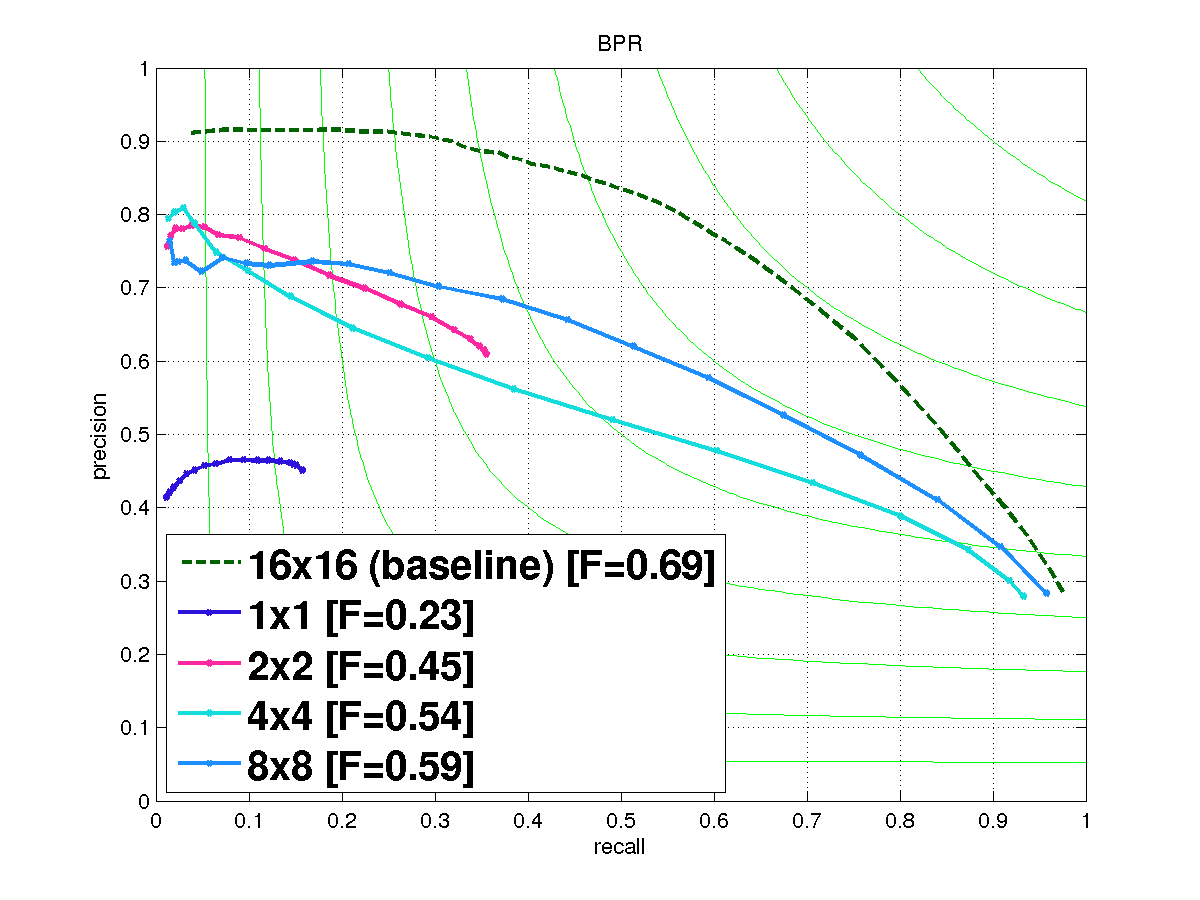
\includegraphics[trim=1.5cm 0cm 1.9cm 0cm, clip=true, width=0.48\textwidth]{images/plots/degraded-baseline_BPR.png}
 }
 \subfigure[VPR]{%
  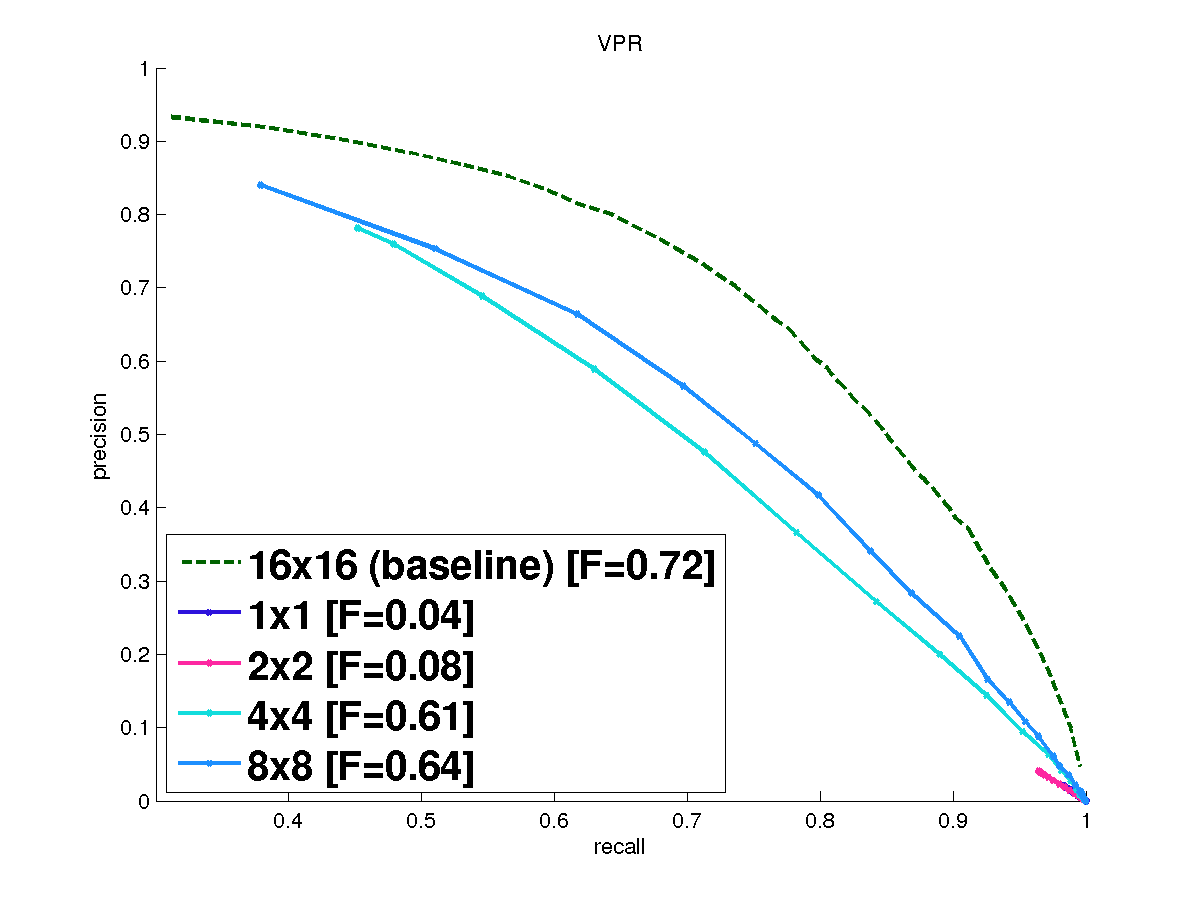
\includegraphics[trim=1.5cm 0cm 1.9cm 0cm, clip=true, width=0.48\textwidth]{images/plots/degraded-baseline_VPR.png}
 }
\caption[Voting scope - reducing the SF patch size - plots]{Voting scope - reducing the SF patch size for the baseline. The original SE-UCM baseline (sref{sec:ch5-SE-UCM-baseline}) uses $16\times16$ pixels output patches. Reducing the patches size proves detrimental to %gravely %greatly diminished
the detector's performance.}
\label{fig:degraded-baseline}
\end{figure}

\subsubsection{Reduced vote scope by dispensing with spatial averaging}
As described in \sref{sec:ch4-SE-SV-UCM_SV_details}, we apportion % NOTE smart word! :-)
the individual votes cast on the watershed contours, by averaging them {\bf per watershed arc}. Apart from increasing the scope of the votes, this has the added benefit of denoising the weighting. 

To confirm % check, make sure
that averaging of the votes is critical for the operation %functioning 
of our SE-SV-UCM pipeline, we dispense with the averaging per intervening edge. We cast just $T$ votes (where $T$ is the number of trees in the decision forest) on a single pixel of the watershed location (we do however average those $T$, in order to associate a score with the pixel location). As expected, that severely diminishes performance in comparison to averaging on the watershed arc. % not region boundary yet
This is due to the reduction of the voting scope to 1 pixel. {\bf Excessive localisation therefore hinders performance}. \fref{fig:reduced-vote-scope} shows the plots resulting from modifying one of our best-performing SV methods: the watershed transformation is fitting a line that adheres to the centre of the patch (as we describe in Section~\ref*{sec:ch4-patch-transformations}~\ref{par:ch4-line-centre}) and the scoring function - VPR normalised on the side of the watershed patch (see Section~\ref*{sec:ch4-boundary-and-region-metrics-maths}~\ref{par:ch4-VPR-maths}).

\begin{figure}[ht!]
\centering
 \subfigure[BPR]{%
  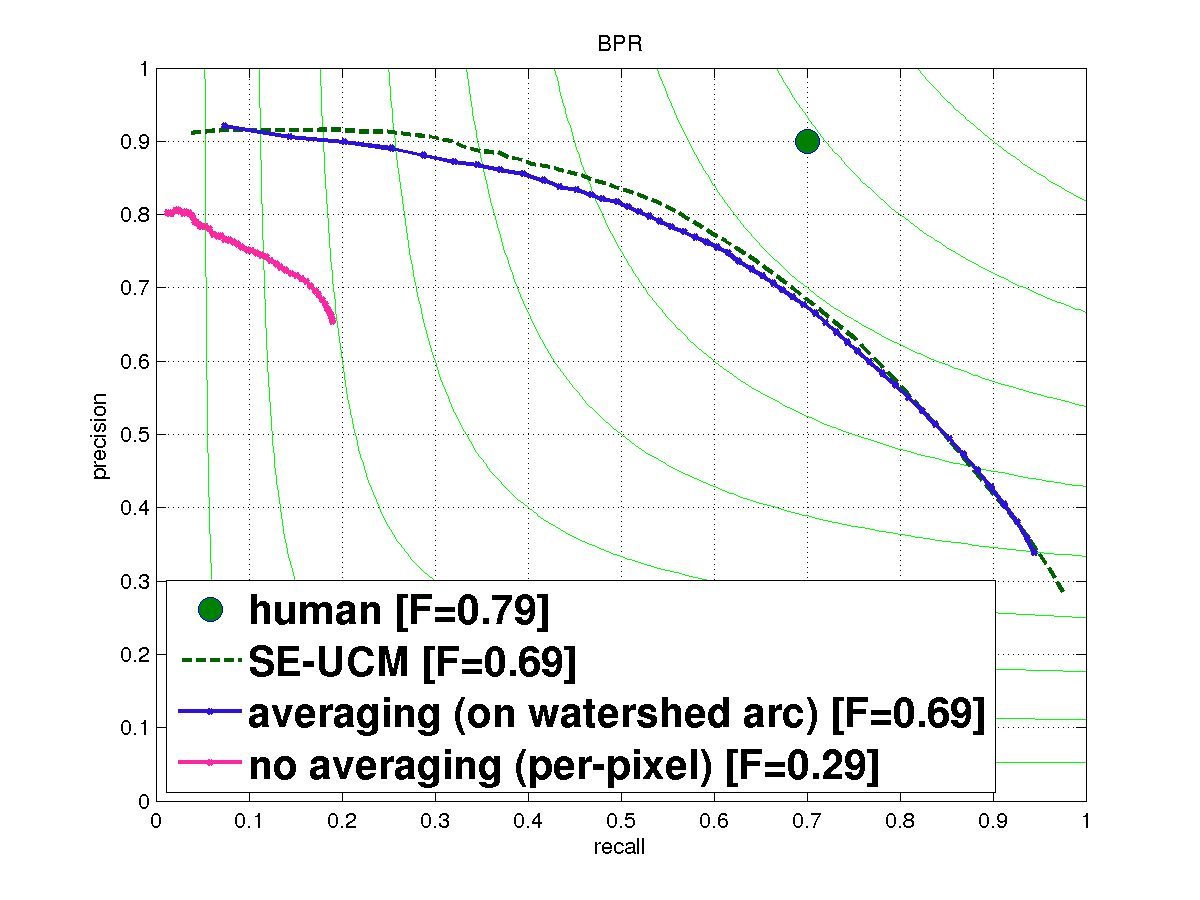
\includegraphics[trim=1.5cm 0cm 1.9cm 0cm, clip=true, width=0.48\textwidth]{images/plots/reduced-vote-scope_BPR.png}
 }
 \subfigure[VPR]{%
  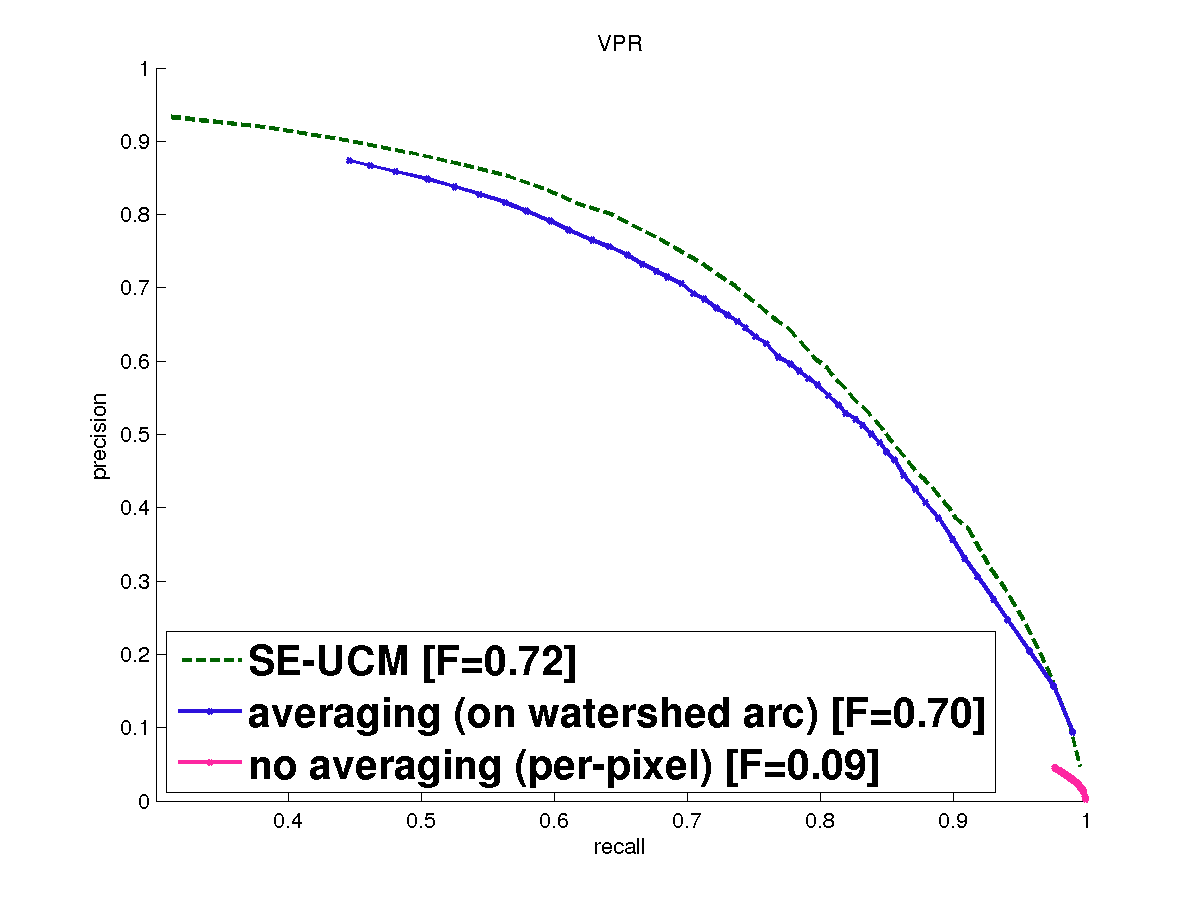
\includegraphics[trim=1.5cm 0cm 1.9cm 0cm, clip=true, width=0.48\textwidth]{images/plots/reduced-vote-scope_VPR.png}
 }
\caption[Voting scope: dispensing with spatial averaging of votes - plots]{Voting scope - dispensing with spatial averaging of votes. The ablated method does not perform any spatial averaging of its votes which consequently damages its performance. See the text for details on this particular method.}
\label{fig:reduced-vote-scope}
\end{figure}

\subsection{Expanding voting scope}
The above two experiments showed us that decreasing the scope of the votes greatly reduces the segmenter's performance. It is therefore natural to seek strategies to expand the voting scope and allow for larger spatial context to be influenced by an individual vote.

In the following we will discuss and modify the central line fitting-VPR method, as it is one of the best that we tried hitherto. So far all experiments used the {\bf watershed arc} as an image edge for both 1) averaging the votes on all pixels from the {\it watershed arc}, and 2) watershed transformation - fitting a line through the patch centre and the end points of the {\it watershed arc}. In the plots \fref{fig:voting-scope-line-centre-VPR-ws} this setup is labelled `arc - arc'.

% from my email 2015-02-10
%
% Before the mid masters presentation votes were cast on subdivided watershed arcs, and those same subdivided edges were used in the watershed transformation. So 'arc - arc' is the scope of voting that we always applied by default.
% 
% Since then, I tried extending the scope of the vote by:
% allowing vote to be cast on larger edge - the whole region boundary ('region boundary - arc'), and still using the subdivided arcs to fit the watershed patch,
% letting the region boundary be used for casting the vote and for transforming the watershed patch ('region boundary - region boundary').
% 
% I get what I call "inconclusive results". I consider the oracle to be a better indicator of the quality of the method than the experiment itself. Indeed, the 3 experiments barely differ both on BPR and VPR. However, in the oracle scenario, I have the best oracle method on BPR metric to be worst on the VPR metric (pink '-.' line).
% 
% I find it therefore hard to draw any definite conclusions or choose scope of voting (among the 3 options).

% Discussion: It would be useful to see the effect of a ``mixed'' scope of voting - cast vote on the whole region boundary, but use subdivided region boundary - the watershed arc in order to do the patch transformation. % UPDATE: it's done!

We extend the scope in two ways:
\begin{enumerate}
 \item{`region boundary - arc'} in \fref{fig:voting-scope-line-centre-VPR-ws}. 1) We extend the edge on which we allow a single vote to influence - it is now the whole intervening {\bf region boundary}, not just the subdivided watershed arc, and 2) we still use the {\bf subdivided arcs} when transforming the watershed patch. 
 \item{`region boundary - region boundary'} in \fref{fig:voting-scope-line-centre-VPR-ws}. We let the {\bf region boundary} be used for both 1) casting the vote and for 2) transforming the watershed patch.
\end{enumerate}


% TODO make oracles plot lines the same colour as the corresponding experiments
\begin{figure}[ht!]
\centering
 \subfigure[BPR]{%
  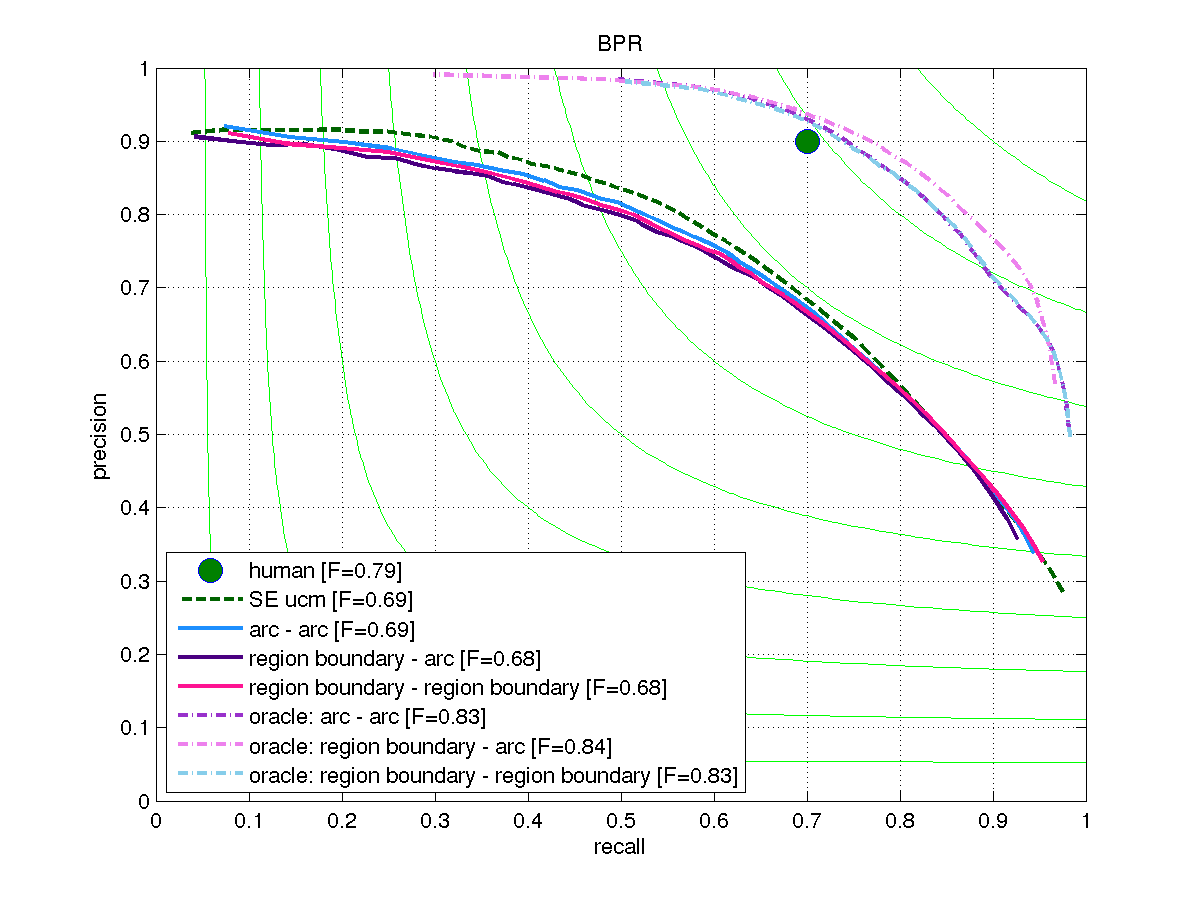
\includegraphics[trim=1.5cm 0cm 1.9cm 0cm, clip=true, width=0.48\textwidth]{images/plots/scope_of_voting_oracle_disagreement__line_centre_VPR_ws_BPR.png}
 }
 \subfigure[VPR]{%
  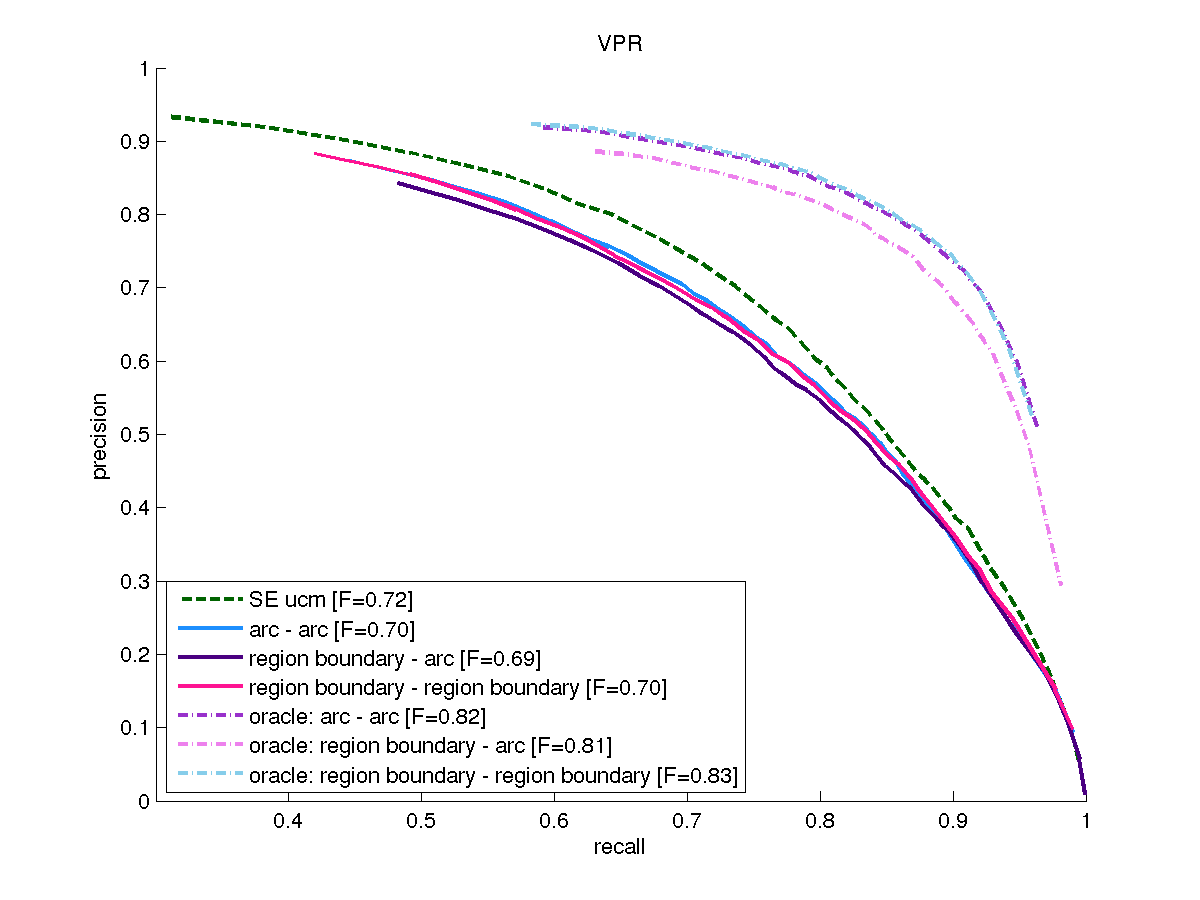
\includegraphics[trim=1.5cm 0cm 1.9cm 0cm, clip=true, width=0.48\textwidth]{images/plots/scope_of_voting_oracle_disagreement__line_centre_VPR_ws_VPR.png}
 }
\caption[Increasing the voting scope - plots]{Results of increasing the voting scope. The three segmentation methods and their oracles are variants of our best performing weighting strategy - central line fitting, combined with VPR normalised on the side of the watershed. A description of VPR is given in Section~\ref*{sec:ch4-boundary-and-region-metrics-maths}~\ref{par:ch4-VPR-maths}).}
\label{fig:voting-scope-line-centre-VPR-ws}
\end{figure}

Results prove to be somewhat inconclusive. Simply judging by the experiments, the `arc - arc' approach is only slightly % not marginally
better than the 2 new methods we tried both on BPR and VPR. We consider, however, the oracle to be a better indicator of the quality of the method. However, in the oracle scenario, the best oracle method on the BPR metric is the worst performing one on the VPR metric (the `oracle: region boundary - arc' method - the pink dashed-and-dotted line in the plots in \fref{fig:voting-scope-line-centre-VPR-ws}).

So deciding between subdivided watershed arc and region boundary for the scope of voting and the watershed transformation is not really crucial for performance and, indeed, place a {\bf minor role} in comparison with other factors like choice of patch transformation and of scoring function.

\section{Discussion}

\tref{tab:all-results} provides comparison with state-of-the art and a detailed report of the results featured in this chapter.
% TODO here is a table of all results we will show. What to do with it, can't just dump all the data without proper analysis / conclusion?
\begin{table}[htbp]
\renewcommand{\arraystretch}{1.3}
\centering
\scriptsize
\begin{tabular}{l|c|c|c||c|c|c||c|c|c|}
\cline{2-10} % ZZ
\multirow{2}{*}{} & \multicolumn{3}{c||}{\textbf{BPR}} & \multicolumn{3}{c||}{\textbf{VPR}}& \multicolumn{3}{c|}{\textbf{Region}}\\
\cline{2-10}
& \textbf{ODS}  & \textbf{OIS} & \textbf{AP} % <- BPR
& \textbf{ODS} & \textbf{OSS} & \textbf{AP} % <- VPR
& \textbf{SC} & \textbf{PRI} & \textbf{VoI} \\
\hline
\multicolumn{1}{|c|}{Human} & .79 & .79 & - & - & - & - & .72 & .88 & 1.17 \\ % actually, we had .80 for humans on BPR from \cite{Arbelaez11}; % TODO for VPR - we don't know ODS = OIS for humans
\hline
\hline
\multicolumn{1}{|c|}{\cite{DollarICCV13edges} Structured edge (SE)} & .70 & .72 & .63 & - & - & - & - & - & - \\
\hline
\multicolumn{1}{|c|}{\cite{Arbelaez11} gPb-OWT-UCM} & .73 & .76 & .77 & .73 & .76 & .78 & .59 & .83 & 1.69 \\
\hline
\hline
\multicolumn{1}{|c|}{SE-watershed} & .39 & .39 & - & .34 & .34 & - & .20 & .75 & 6.26 \\
\hline
\multicolumn{1}{|c|}{SE-UCM (baseline)} & .69 &.73 & .75 & .72 & .75 & .77 & .58 & .82 & 1.80 \\
\hline
\multicolumn{1}{|c|}{SE+sPb-UCM} & .72 & .75 & .76 & .73 & .76 & .78 & .59 & .82 & 1.68 \\ % SE_nnms_sPb-UCM
\hline
\hline
\multicolumn{1}{|c|}{linear LLS} & .68 & .71 & .71 & .69 & .71 & .71 & .55 & .81 & 1.90 \\% linear model - linear least squares fitting}
\hline
\multicolumn{1}{|c|}{quadratic LLS} & .54 & .56 & .40 & .40 & .40 & .25 & .37 & .55 & 2.45 \\
\hline
\hline
\end{tabular}
\caption[All results]{Results of all our experiments.}
%The table shows aggregate measures (ODS, OSS, AP) for boundary precision-recall (BPR), volume precision-recall (VPR) and 
%includes region statistics (SC, PRI, VoI).}
\label{tab:all-results}
\end{table}

% quadratic
% Boundary PR global
%    G-ODS: F( R 0.57, P 0.52 ) = 0.54   [th = 0.12]
%    G-OIS: F( R 0.57, P 0.54 ) = 0.56
%    Area_PR = 0.40
% Volume PR global
%    G-ODS: F( R 0.79, P 0.27 ) = 0.40   [th = 0.02]            <- NOTE: very low threshold! can't recall all boundaries, that explains the plot
%    G-OSS: F( R 0.79, P 0.26 ) = 0.40
%    G-Area_PR = 0.25
% Region
%    GT covering: ODS = 0.34 [th = 0.21]. OSS = 0.35. Best = 0.37
% Region
%    Rand Index: ODS = 0.55 [th = 0.02]. OSS = 0.55.
%    Var. Info.: ODS = 2.45 [th = 0.73]. OSS = 2.37.


% SE-UCM baseline
% Boundary PR global
%    G-ODS: F( R 0.70, P 0.69 ) = 0.69   [th = 0.27]
%    G-OIS: F( R 0.73, P 0.73 ) = 0.73
%    Area_PR = 0.75
% Volume PR global
%    G-ODS: F( R 0.71, P 0.73 ) = 0.72   [th = 0.25]
%    G-OSS: F( R 0.73, P 0.77 ) = 0.75
%    G-Area_PR = 0.77
% Region
%    GT covering: ODS = 0.58 [th = 0.29]. OSS = 0.64. Best = 0.73
% Region
%    Rand Index: ODS = 0.82 [th = 0.17]. OSS = 0.86.
%    Var. Info.: ODS = 1.80 [th = 0.52]. OSS = 1.57.

% SE_nnms_sPb-UCM
% Boundary PR global
%    G-ODS: F( R 0.72, P 0.72 ) = 0.72   [th = 0.08]
%    G-OIS: F( R 0.74, P 0.76 ) = 0.75
%    Area_PR = 0.76
% Volume PR global
%    G-ODS: F( R 0.70, P 0.76 ) = 0.73   [th = 0.10]
%    G-OSS: F( R 0.74, P 0.77 ) = 0.76
%    G-Area_PR = 0.78
% Region
%    GT covering: ODS = 0.59 [th = 0.12]. OSS = 0.64. Best = 0.74
% Region
%    Rand Index: ODS = 0.82 [th = 0.08]. OSS = 0.85.
%    Var. Info.: ODS = 1.68 [th = 0.15]. OSS = 1.48.

% linear LLS
% Boundary PR global
%    G-ODS: F( R 0.69, P 0.67 ) = 0.68   [th = 0.35]
%    G-OIS: F( R 0.74, P 0.67 ) = 0.71
%    Area_PR = 0.71
% Volume PR global
%    G-ODS: F( R 0.68, P 0.70 ) = 0.69   [th = 0.27]
%    G-OSS: F( R 0.70, P 0.73 ) = 0.71
%    G-Area_PR = 0.71
% Region
%    GT covering: ODS = 0.55 [th = 0.37]. OSS = 0.60. Best = 0.67
% Region
%    Rand Index: ODS = 0.81 [th = 0.17]. OSS = 0.83.
%    Var. Info.: ODS = 1.90 [th = 0.67]. OSS = 1.72.

% quadratic LLS
% Boundary PR global
%    G-ODS: F( R 0.57, P 0.52 ) = 0.54   [th = 0.12]
%    G-OIS: F( R 0.57, P 0.54 ) = 0.56
%    Area_PR = 0.40
% Volume PR global
%    G-ODS: F( R 0.79, P 0.27 ) = 0.40   [th = 0.02]
%    G-OSS: F( R 0.79, P 0.26 ) = 0.40
%    G-Area_PR = 0.25
% Region
%    GT covering: ODS = 0.34 [th = 0.21]. OSS = 0.35. Best = 0.37


Important conclusions of the experiments:
\begin{enumerate}
 \item both watershed transformations and scoring functions are important,
 % \item scoring functions matter,
 \item a suitable %smart
 watershed transformation could greatly aid a ``weaker'' scoring function (\eg the benefit of greedy merge when using RI scoring function),
 \item our best watershed transformation has reasonable performance with all the scoring functions tried,
 \item oracle confirms the ranking of our experiments,
 \item simpler models work better for transforming the watershed patch (\eg quadratic and polynomial fitting are the worst performing experiments regardless of the scoring function used),
 \item voting scope is very important; a decrease in the voting scope seriously damages results; successfully increasing the voting scope is not trivial.
\end{enumerate}